% Generated by Sphinx.
\def\sphinxdocclass{report}
\documentclass[letterpaper,10pt,english]{sphinxmanual}
\usepackage[utf8]{inputenc}
\DeclareUnicodeCharacter{00A0}{\nobreakspace}
\usepackage{cmap}
\usepackage[T1]{fontenc}
\usepackage{babel}
\usepackage{times}
\usepackage[Bjarne]{fncychap}
\usepackage{longtable}
\usepackage{sphinx}
\usepackage{multirow}

\addto\captionsenglish{\renewcommand{\figurename}{Fig. }}
\addto\captionsenglish{\renewcommand{\tablename}{Table }}
\floatname{literal-block}{Listing }



\title{AOIC}
\date{June 11, 2015}
\release{1.0 beta}
\author{}
\newcommand{\sphinxlogo}{}
\renewcommand{\releasename}{Release}
\makeindex

\makeatletter
\def\PYG@reset{\let\PYG@it=\relax \let\PYG@bf=\relax%
    \let\PYG@ul=\relax \let\PYG@tc=\relax%
    \let\PYG@bc=\relax \let\PYG@ff=\relax}
\def\PYG@tok#1{\csname PYG@tok@#1\endcsname}
\def\PYG@toks#1+{\ifx\relax#1\empty\else%
    \PYG@tok{#1}\expandafter\PYG@toks\fi}
\def\PYG@do#1{\PYG@bc{\PYG@tc{\PYG@ul{%
    \PYG@it{\PYG@bf{\PYG@ff{#1}}}}}}}
\def\PYG#1#2{\PYG@reset\PYG@toks#1+\relax+\PYG@do{#2}}

\expandafter\def\csname PYG@tok@gd\endcsname{\def\PYG@tc##1{\textcolor[rgb]{0.63,0.00,0.00}{##1}}}
\expandafter\def\csname PYG@tok@gu\endcsname{\let\PYG@bf=\textbf\def\PYG@tc##1{\textcolor[rgb]{0.50,0.00,0.50}{##1}}}
\expandafter\def\csname PYG@tok@gt\endcsname{\def\PYG@tc##1{\textcolor[rgb]{0.00,0.27,0.87}{##1}}}
\expandafter\def\csname PYG@tok@gs\endcsname{\let\PYG@bf=\textbf}
\expandafter\def\csname PYG@tok@gr\endcsname{\def\PYG@tc##1{\textcolor[rgb]{1.00,0.00,0.00}{##1}}}
\expandafter\def\csname PYG@tok@cm\endcsname{\let\PYG@it=\textit\def\PYG@tc##1{\textcolor[rgb]{0.25,0.50,0.56}{##1}}}
\expandafter\def\csname PYG@tok@vg\endcsname{\def\PYG@tc##1{\textcolor[rgb]{0.73,0.38,0.84}{##1}}}
\expandafter\def\csname PYG@tok@m\endcsname{\def\PYG@tc##1{\textcolor[rgb]{0.13,0.50,0.31}{##1}}}
\expandafter\def\csname PYG@tok@mh\endcsname{\def\PYG@tc##1{\textcolor[rgb]{0.13,0.50,0.31}{##1}}}
\expandafter\def\csname PYG@tok@cs\endcsname{\def\PYG@tc##1{\textcolor[rgb]{0.25,0.50,0.56}{##1}}\def\PYG@bc##1{\setlength{\fboxsep}{0pt}\colorbox[rgb]{1.00,0.94,0.94}{\strut ##1}}}
\expandafter\def\csname PYG@tok@ge\endcsname{\let\PYG@it=\textit}
\expandafter\def\csname PYG@tok@vc\endcsname{\def\PYG@tc##1{\textcolor[rgb]{0.73,0.38,0.84}{##1}}}
\expandafter\def\csname PYG@tok@il\endcsname{\def\PYG@tc##1{\textcolor[rgb]{0.13,0.50,0.31}{##1}}}
\expandafter\def\csname PYG@tok@go\endcsname{\def\PYG@tc##1{\textcolor[rgb]{0.20,0.20,0.20}{##1}}}
\expandafter\def\csname PYG@tok@cp\endcsname{\def\PYG@tc##1{\textcolor[rgb]{0.00,0.44,0.13}{##1}}}
\expandafter\def\csname PYG@tok@gi\endcsname{\def\PYG@tc##1{\textcolor[rgb]{0.00,0.63,0.00}{##1}}}
\expandafter\def\csname PYG@tok@gh\endcsname{\let\PYG@bf=\textbf\def\PYG@tc##1{\textcolor[rgb]{0.00,0.00,0.50}{##1}}}
\expandafter\def\csname PYG@tok@ni\endcsname{\let\PYG@bf=\textbf\def\PYG@tc##1{\textcolor[rgb]{0.84,0.33,0.22}{##1}}}
\expandafter\def\csname PYG@tok@nl\endcsname{\let\PYG@bf=\textbf\def\PYG@tc##1{\textcolor[rgb]{0.00,0.13,0.44}{##1}}}
\expandafter\def\csname PYG@tok@nn\endcsname{\let\PYG@bf=\textbf\def\PYG@tc##1{\textcolor[rgb]{0.05,0.52,0.71}{##1}}}
\expandafter\def\csname PYG@tok@no\endcsname{\def\PYG@tc##1{\textcolor[rgb]{0.38,0.68,0.84}{##1}}}
\expandafter\def\csname PYG@tok@na\endcsname{\def\PYG@tc##1{\textcolor[rgb]{0.25,0.44,0.63}{##1}}}
\expandafter\def\csname PYG@tok@nb\endcsname{\def\PYG@tc##1{\textcolor[rgb]{0.00,0.44,0.13}{##1}}}
\expandafter\def\csname PYG@tok@nc\endcsname{\let\PYG@bf=\textbf\def\PYG@tc##1{\textcolor[rgb]{0.05,0.52,0.71}{##1}}}
\expandafter\def\csname PYG@tok@nd\endcsname{\let\PYG@bf=\textbf\def\PYG@tc##1{\textcolor[rgb]{0.33,0.33,0.33}{##1}}}
\expandafter\def\csname PYG@tok@ne\endcsname{\def\PYG@tc##1{\textcolor[rgb]{0.00,0.44,0.13}{##1}}}
\expandafter\def\csname PYG@tok@nf\endcsname{\def\PYG@tc##1{\textcolor[rgb]{0.02,0.16,0.49}{##1}}}
\expandafter\def\csname PYG@tok@si\endcsname{\let\PYG@it=\textit\def\PYG@tc##1{\textcolor[rgb]{0.44,0.63,0.82}{##1}}}
\expandafter\def\csname PYG@tok@s2\endcsname{\def\PYG@tc##1{\textcolor[rgb]{0.25,0.44,0.63}{##1}}}
\expandafter\def\csname PYG@tok@vi\endcsname{\def\PYG@tc##1{\textcolor[rgb]{0.73,0.38,0.84}{##1}}}
\expandafter\def\csname PYG@tok@nt\endcsname{\let\PYG@bf=\textbf\def\PYG@tc##1{\textcolor[rgb]{0.02,0.16,0.45}{##1}}}
\expandafter\def\csname PYG@tok@nv\endcsname{\def\PYG@tc##1{\textcolor[rgb]{0.73,0.38,0.84}{##1}}}
\expandafter\def\csname PYG@tok@s1\endcsname{\def\PYG@tc##1{\textcolor[rgb]{0.25,0.44,0.63}{##1}}}
\expandafter\def\csname PYG@tok@gp\endcsname{\let\PYG@bf=\textbf\def\PYG@tc##1{\textcolor[rgb]{0.78,0.36,0.04}{##1}}}
\expandafter\def\csname PYG@tok@sh\endcsname{\def\PYG@tc##1{\textcolor[rgb]{0.25,0.44,0.63}{##1}}}
\expandafter\def\csname PYG@tok@ow\endcsname{\let\PYG@bf=\textbf\def\PYG@tc##1{\textcolor[rgb]{0.00,0.44,0.13}{##1}}}
\expandafter\def\csname PYG@tok@sx\endcsname{\def\PYG@tc##1{\textcolor[rgb]{0.78,0.36,0.04}{##1}}}
\expandafter\def\csname PYG@tok@bp\endcsname{\def\PYG@tc##1{\textcolor[rgb]{0.00,0.44,0.13}{##1}}}
\expandafter\def\csname PYG@tok@c1\endcsname{\let\PYG@it=\textit\def\PYG@tc##1{\textcolor[rgb]{0.25,0.50,0.56}{##1}}}
\expandafter\def\csname PYG@tok@kc\endcsname{\let\PYG@bf=\textbf\def\PYG@tc##1{\textcolor[rgb]{0.00,0.44,0.13}{##1}}}
\expandafter\def\csname PYG@tok@c\endcsname{\let\PYG@it=\textit\def\PYG@tc##1{\textcolor[rgb]{0.25,0.50,0.56}{##1}}}
\expandafter\def\csname PYG@tok@mf\endcsname{\def\PYG@tc##1{\textcolor[rgb]{0.13,0.50,0.31}{##1}}}
\expandafter\def\csname PYG@tok@err\endcsname{\def\PYG@bc##1{\setlength{\fboxsep}{0pt}\fcolorbox[rgb]{1.00,0.00,0.00}{1,1,1}{\strut ##1}}}
\expandafter\def\csname PYG@tok@mb\endcsname{\def\PYG@tc##1{\textcolor[rgb]{0.13,0.50,0.31}{##1}}}
\expandafter\def\csname PYG@tok@ss\endcsname{\def\PYG@tc##1{\textcolor[rgb]{0.32,0.47,0.09}{##1}}}
\expandafter\def\csname PYG@tok@sr\endcsname{\def\PYG@tc##1{\textcolor[rgb]{0.14,0.33,0.53}{##1}}}
\expandafter\def\csname PYG@tok@mo\endcsname{\def\PYG@tc##1{\textcolor[rgb]{0.13,0.50,0.31}{##1}}}
\expandafter\def\csname PYG@tok@kd\endcsname{\let\PYG@bf=\textbf\def\PYG@tc##1{\textcolor[rgb]{0.00,0.44,0.13}{##1}}}
\expandafter\def\csname PYG@tok@mi\endcsname{\def\PYG@tc##1{\textcolor[rgb]{0.13,0.50,0.31}{##1}}}
\expandafter\def\csname PYG@tok@kn\endcsname{\let\PYG@bf=\textbf\def\PYG@tc##1{\textcolor[rgb]{0.00,0.44,0.13}{##1}}}
\expandafter\def\csname PYG@tok@o\endcsname{\def\PYG@tc##1{\textcolor[rgb]{0.40,0.40,0.40}{##1}}}
\expandafter\def\csname PYG@tok@kr\endcsname{\let\PYG@bf=\textbf\def\PYG@tc##1{\textcolor[rgb]{0.00,0.44,0.13}{##1}}}
\expandafter\def\csname PYG@tok@s\endcsname{\def\PYG@tc##1{\textcolor[rgb]{0.25,0.44,0.63}{##1}}}
\expandafter\def\csname PYG@tok@kp\endcsname{\def\PYG@tc##1{\textcolor[rgb]{0.00,0.44,0.13}{##1}}}
\expandafter\def\csname PYG@tok@w\endcsname{\def\PYG@tc##1{\textcolor[rgb]{0.73,0.73,0.73}{##1}}}
\expandafter\def\csname PYG@tok@kt\endcsname{\def\PYG@tc##1{\textcolor[rgb]{0.56,0.13,0.00}{##1}}}
\expandafter\def\csname PYG@tok@sc\endcsname{\def\PYG@tc##1{\textcolor[rgb]{0.25,0.44,0.63}{##1}}}
\expandafter\def\csname PYG@tok@sb\endcsname{\def\PYG@tc##1{\textcolor[rgb]{0.25,0.44,0.63}{##1}}}
\expandafter\def\csname PYG@tok@k\endcsname{\let\PYG@bf=\textbf\def\PYG@tc##1{\textcolor[rgb]{0.00,0.44,0.13}{##1}}}
\expandafter\def\csname PYG@tok@se\endcsname{\let\PYG@bf=\textbf\def\PYG@tc##1{\textcolor[rgb]{0.25,0.44,0.63}{##1}}}
\expandafter\def\csname PYG@tok@sd\endcsname{\let\PYG@it=\textit\def\PYG@tc##1{\textcolor[rgb]{0.25,0.44,0.63}{##1}}}

\def\PYGZbs{\char`\\}
\def\PYGZus{\char`\_}
\def\PYGZob{\char`\{}
\def\PYGZcb{\char`\}}
\def\PYGZca{\char`\^}
\def\PYGZam{\char`\&}
\def\PYGZlt{\char`\<}
\def\PYGZgt{\char`\>}
\def\PYGZsh{\char`\#}
\def\PYGZpc{\char`\%}
\def\PYGZdl{\char`\$}
\def\PYGZhy{\char`\-}
\def\PYGZsq{\char`\'}
\def\PYGZdq{\char`\"}
\def\PYGZti{\char`\~}
% for compatibility with earlier versions
\def\PYGZat{@}
\def\PYGZlb{[}
\def\PYGZrb{]}
\makeatother

\renewcommand\PYGZsq{\textquotesingle}

\begin{document}

\maketitle
\tableofcontents
\phantomsection\label{index::doc}



\chapter{Overview}
\label{overview:overview}\label{overview::doc}\label{overview:aoic-documentation}
\textsc{AOIC} (ANOPP2 OpenMDAO Interface Code) is an interface code written in Python developed at \textsc{NASA} (National Aeronautics and Space Administration) \textsc{LaRC} (Langley Research Center) that offers an ability to use \textsc{ANOPP2} (Aircraft NOise Prediction Program 2) to optimize designs using \textsc{OpenMDAO} (Open Multi-disciplinary Design Analysis and Optimization).
The AOIC contains two classes: the first interacts with ANOPP2 for setting the problem to be optimized and the second specifies the conditions for optimization.
The AOIC developed to solve a simple case of finding the location of maximum noise along a sideline parallel to the flight path during an aircraft takeoff is provided and explained.

\index{ANOPP2}
\index{ANOPP}
\index{AOIC}
\index{Noise Prediction}

\chapter{Introduction}
\label{introduction:introduction}\label{introduction::doc}\label{introduction:index-3}
Aircraft design has traditionally been based on performance characteristics, carrying capacity, and operational efficiency.
With FAA's increasingly stringent specifications on aircraft noise, aircraft designers are increasing the importance of aircraft noise in their designs.
Design engineers can use \textsc{OpenMDAO} to arrive at a combination of various design variables that optimizes several performance characteristics.
\textsc{ANOPP2} is a tool available to aircraft design engineers for predicting noise from the aircraft at various observer locations.
\textsc{AOIC} is an interface code, written in Python, between ANOPP2 and OpenMDAO for the purpose of minimizing aircraft noise.
Aircraft design engineers can include noise as one of the parameters to be optimized by using AOIC to bring aircraft noise, predicted by ANOPP2, into OpenMDAO.
A demonstration case is provided that predicts sideline noise during takeoff for the purpose of demonstrating the functionality of the AOIC.
During takeoff, one of the certification microphone locations is on the sideline, measured in terms of \textsc{EPNL} (Effective Perceived Noise Level).
The sideline microphone location should be at the maximum noise location; this sample case demonstrates the use of AOIC to determine this location.


\chapter{Requirements}
\label{requirements:requirements}\label{requirements::doc}
\textsc{AOIC} requires the installation of OpenMDAO in addition to Python 2.7 along with the numerical and scientific packages NumPy and SciPy. AOIC is a Python plugin in OpenMDAO that the user will have to create to use ANOPP2 for noise optimization. AOIC also requires library, \code{libANOPP2.so}, and the ANOPP2 API, \code{ANOPP2\_api.py}.


\chapter{Usage Guide}
\label{usage:usage-guide}\label{usage::doc}
The \textsc{AOIC} contains two classes: \emph{Anopp2Component} and \emph{Anopp2Optimize}.
The \emph{Anopp2Component} class contains the essence of all interactions with ANOPP2.
Details of the \emph{Anopp2Component} class used in this specific example are provided herein.
Users desiring to use ANOPP2 for optimization through OpenMDAO are required to develop similar codes with appropriate ANOPP2 function calls and other necessary associated files (see ANOPP2 Manuals for more information).
This example code is tested through a test code, \emph{test\_anopp2.py}.

In this case, the noise generated during the takeoff of a \emph{Tube and Wing} aircraft is modeled through ANOPP2 and the noise along a sideline parallel to the takeoff direction on the ground is predicted.
The location along the sideline at which the noise (measured through the acoustic metric \textsc{EPNL}) reaches its maximum is determined through OpenMDAO.
The details of this \textsc{AOIC} are explained here.


\section{Anopp2Component}
\label{usage:anopp2component}

\subsection{Initialization}
\label{usage:initialization}
\textbf{Step 1. Initialize ANOPP2 API}: The ANOPP2 Command Executive API {[}{\hyperref[usage:lopes2014a]{\emph{LOPES2014A}}}{]} is initialized first through the following command: \code{ANOPP2.a2py\_exec\_init\_api ()}.

\textbf{Step 2. Initialize local variables}: Initialize the Atmosphere and Flight Path tags.

\textbf{Step 3. Create an Observer}: An observer {[}{\hyperref[usage:lopes2014b]{\emph{LOPES2014B}}}{]} is defined as a point cloud (a collection of several points in space, also referred to as \emph{nodes}) along the sideline defined by its x (along the direction of the flight on the ground), y (perpendicular to the direction of flight on the ground), and z (perpendicular to the ground) axes. The observer is defined in a configuration file, \emph{observer.config} placed in the current working folder.  This configuration file is provided below:

\begin{Verbatim}[commandchars=\\\{\},numbers=left,firstnumber=1,stepnumber=1]
!\PYGZhy{}\PYGZhy{}\PYGZhy{}\PYGZhy{}\PYGZhy{}\PYGZhy{}\PYGZhy{}\PYGZhy{}\PYGZhy{}\PYGZhy{}\PYGZhy{}\PYGZhy{}\PYGZhy{}\PYGZhy{}\PYGZhy{}\PYGZhy{}\PYGZhy{}\PYGZhy{}\PYGZhy{}\PYGZhy{}\PYGZhy{}\PYGZhy{}\PYGZhy{}\PYGZhy{}\PYGZhy{}\PYGZhy{}\PYGZhy{}\PYGZhy{}\PYGZhy{}\PYGZhy{}\PYGZhy{}\PYGZhy{}\PYGZhy{}\PYGZhy{}\PYGZhy{}\PYGZhy{}\PYGZhy{}\PYGZhy{}\PYGZhy{}\PYGZhy{}\PYGZhy{}\PYGZhy{}\PYGZhy{}\PYGZhy{}\PYGZhy{}\PYGZhy{}\PYGZhy{}\PYGZhy{}\PYGZhy{}\PYGZhy{}\PYGZhy{}\PYGZhy{}\PYGZhy{}\PYGZhy{}\PYGZhy{}\PYGZhy{}\PYGZhy{}\PYGZhy{}\PYGZhy{}\PYGZhy{}\PYGZhy{}\PYGZhy{}\PYGZhy{}\PYGZhy{}\PYGZhy{}\PYGZhy{}\PYGZhy{}\PYGZhy{}\PYGZhy{}\PYGZhy{}\PYGZhy{}\PYGZhy{}\PYGZhy{}\PYGZhy{}\PYGZhy{}\PYGZhy{}\PYGZhy{}\PYGZhy{}\PYGZhy{}\PYGZhy{}\PYGZhy{}\PYGZhy{}\PYGZhy{}\PYGZhy{}
! This is the namelist that defines the ground observer positions that will be passed 
! to ANOPP during execution.  This configuration is for several observer positions 
! along the sideline of a takeoff flightpath.
!\PYGZhy{}\PYGZhy{}\PYGZhy{}\PYGZhy{}\PYGZhy{}\PYGZhy{}\PYGZhy{}\PYGZhy{}\PYGZhy{}\PYGZhy{}\PYGZhy{}\PYGZhy{}\PYGZhy{}\PYGZhy{}\PYGZhy{}\PYGZhy{}\PYGZhy{}\PYGZhy{}\PYGZhy{}\PYGZhy{}\PYGZhy{}\PYGZhy{}\PYGZhy{}\PYGZhy{}\PYGZhy{}\PYGZhy{}\PYGZhy{}\PYGZhy{}\PYGZhy{}\PYGZhy{}\PYGZhy{}\PYGZhy{}\PYGZhy{}\PYGZhy{}\PYGZhy{}\PYGZhy{}\PYGZhy{}\PYGZhy{}\PYGZhy{}\PYGZhy{}\PYGZhy{}\PYGZhy{}\PYGZhy{}\PYGZhy{}\PYGZhy{}\PYGZhy{}\PYGZhy{}\PYGZhy{}\PYGZhy{}\PYGZhy{}\PYGZhy{}\PYGZhy{}\PYGZhy{}\PYGZhy{}\PYGZhy{}\PYGZhy{}\PYGZhy{}\PYGZhy{}\PYGZhy{}\PYGZhy{}\PYGZhy{}\PYGZhy{}\PYGZhy{}\PYGZhy{}\PYGZhy{}\PYGZhy{}\PYGZhy{}\PYGZhy{}\PYGZhy{}\PYGZhy{}\PYGZhy{}\PYGZhy{}\PYGZhy{}\PYGZhy{}\PYGZhy{}\PYGZhy{}\PYGZhy{}\PYGZhy{}\PYGZhy{}\PYGZhy{}\PYGZhy{}\PYGZhy{}\PYGZhy{}\PYGZhy{}
\PYGZam{}ObserverPointCloudNamelist
 
  ! Since our microphone is stationary, this parameter is 0, meaning the microphone 
  ! is not moving within the ground frame of reference.
  nFrameChanges = 0

/
  !\PYGZhy{}\PYGZhy{}\PYGZhy{}\PYGZhy{}\PYGZhy{}\PYGZhy{}\PYGZhy{}\PYGZhy{}\PYGZhy{}\PYGZhy{}\PYGZhy{}\PYGZhy{}\PYGZhy{}\PYGZhy{}\PYGZhy{}\PYGZhy{}\PYGZhy{}\PYGZhy{}\PYGZhy{}\PYGZhy{}\PYGZhy{}\PYGZhy{}\PYGZhy{}\PYGZhy{}\PYGZhy{}\PYGZhy{}\PYGZhy{}\PYGZhy{}\PYGZhy{}\PYGZhy{}\PYGZhy{}\PYGZhy{}\PYGZhy{}\PYGZhy{}\PYGZhy{}\PYGZhy{}\PYGZhy{}\PYGZhy{}\PYGZhy{}\PYGZhy{}\PYGZhy{}\PYGZhy{}\PYGZhy{}\PYGZhy{}\PYGZhy{}\PYGZhy{}\PYGZhy{}\PYGZhy{}\PYGZhy{}\PYGZhy{}\PYGZhy{}\PYGZhy{}\PYGZhy{}\PYGZhy{}\PYGZhy{}\PYGZhy{}\PYGZhy{}\PYGZhy{}\PYGZhy{}\PYGZhy{}\PYGZhy{}\PYGZhy{}\PYGZhy{}\PYGZhy{}\PYGZhy{}\PYGZhy{}\PYGZhy{}\PYGZhy{}\PYGZhy{}\PYGZhy{}\PYGZhy{}\PYGZhy{}\PYGZhy{}\PYGZhy{}\PYGZhy{}\PYGZhy{}\PYGZhy{}\PYGZhy{}\PYGZhy{}\PYGZhy{}\PYGZhy{}\PYGZhy{}
  ! The point will be anywhere along the sideline of the takeoff maneuver.  The line 
  ! is 1476 feet (or 449.8848 meters) to the side of the flight path.  The OpenMDAO 
  ! is expected to locate the the observer position at which maximum EPNdB is found. 
  !\PYGZhy{}\PYGZhy{}\PYGZhy{}\PYGZhy{}\PYGZhy{}\PYGZhy{}\PYGZhy{}\PYGZhy{}\PYGZhy{}\PYGZhy{}\PYGZhy{}\PYGZhy{}\PYGZhy{}\PYGZhy{}\PYGZhy{}\PYGZhy{}\PYGZhy{}\PYGZhy{}\PYGZhy{}\PYGZhy{}\PYGZhy{}\PYGZhy{}\PYGZhy{}\PYGZhy{}\PYGZhy{}\PYGZhy{}\PYGZhy{}\PYGZhy{}\PYGZhy{}\PYGZhy{}\PYGZhy{}\PYGZhy{}\PYGZhy{}\PYGZhy{}\PYGZhy{}\PYGZhy{}\PYGZhy{}\PYGZhy{}\PYGZhy{}\PYGZhy{}\PYGZhy{}\PYGZhy{}\PYGZhy{}\PYGZhy{}\PYGZhy{}\PYGZhy{}\PYGZhy{}\PYGZhy{}\PYGZhy{}\PYGZhy{}\PYGZhy{}\PYGZhy{}\PYGZhy{}\PYGZhy{}\PYGZhy{}\PYGZhy{}\PYGZhy{}\PYGZhy{}\PYGZhy{}\PYGZhy{}\PYGZhy{}\PYGZhy{}\PYGZhy{}\PYGZhy{}\PYGZhy{}\PYGZhy{}\PYGZhy{}\PYGZhy{}\PYGZhy{}\PYGZhy{}\PYGZhy{}\PYGZhy{}\PYGZhy{}\PYGZhy{}\PYGZhy{}\PYGZhy{}\PYGZhy{}\PYGZhy{}\PYGZhy{}\PYGZhy{}\PYGZhy{}\PYGZhy{}
  \PYGZam{}PointCloudNamelist
  
    ! This is the number of nodes.
    nNodes = 1
    
  /
  2410.0, 449.8848, 0.0
\end{Verbatim}

The observer is created through the following ANOPP2 command:

\begin{Verbatim}[commandchars=\\\{\}]
\PYG{n}{intSuccess} \PYG{o}{=}             \PYGZbs{}
  \PYG{n}{ANOPP2}\PYG{o}{.}\PYG{n}{a2py\PYGZus{}obs\PYGZus{}create} \PYGZbs{}
   \PYG{p}{(}\PYG{n}{pointer}\PYG{p}{(}\PYG{n+nb+bp}{self}\PYG{o}{.}\PYG{n}{intObserverTag}\PYG{p}{)}\PYG{p}{,} \PYG{n}{create\PYGZus{}string\PYGZus{}buffer} \PYG{p}{(}\PYG{n}{b}\PYG{l+s}{\PYGZdq{}}\PYG{l+s}{observer.config}\PYG{l+s}{\PYGZdq{}}\PYG{p}{)}\PYG{p}{)}
\end{Verbatim}


\subsection{Execution}
\label{usage:execution}
The \emph{Anopp2.py} performs the following steps as part of its execution.
Each of these steps are executed for each iteration to determine the noise (EPNL) corresponding to that observer location.

\textbf{Step 4. Create a New Observer Node}: A new node is introduced into the observer at a location whose \code{x} coordinate is provided by the optimizer and the \code{y} and \code{z} coordinates are those of the previous node.
So, the number of nodes in the observer is first obtained through the following function call:

\begin{Verbatim}[commandchars=\\\{\}]
\PYG{n}{intSuccess} \PYG{o}{=} \PYG{n}{ANOPP2}\PYG{o}{.}\PYG{n}{a2py\PYGZus{}obs\PYGZus{}number\PYGZus{}of\PYGZus{}nodes} \PYG{p}{(}\PYG{n+nb+bp}{self}\PYG{o}{.}\PYG{n}{intObserverTag}\PYG{p}{,} \PYG{n+nb+bp}{self}\PYG{o}{.}\PYG{n}{nNodes}\PYG{p}{)}
\end{Verbatim}

The position of the last node in the observer is obtained through the following function call:

\begin{Verbatim}[commandchars=\\\{\}]
\PYG{n}{intSuccess} \PYG{o}{=}               \PYGZbs{}
  \PYG{n}{ANOPP2}\PYG{o}{.}\PYG{n}{a2py\PYGZus{}obs\PYGZus{}position} \PYGZbs{}
    \PYG{p}{(}\PYG{n+nb+bp}{self}\PYG{o}{.}\PYG{n}{intObserverTag}\PYG{p}{,} \PYG{n+nb+bp}{self}\PYG{o}{.}\PYG{n}{nNodes}\PYG{p}{,} \PYG{l+m+mf}{0.0}\PYG{p}{,} \PYG{n}{a2\PYGZus{}global}\PYG{p}{,} \PYG{n+nb+bp}{self}\PYG{o}{.}\PYG{n}{fltPosition}\PYG{p}{)}
\end{Verbatim}

where, \code{self.fltPosition} is an array containing the \code{x}, \code{y}, and \code{z} coordinates of the position of the last node in the observer.

The first value of the Position array (x coordinate) is replaced with the value provided by the optimizer: \code{self.fltPosition{[}0{]} = self.x}.
A new node is added in the observer point cloud at the location corresponding to the values of the \code{fltPosition} array through the following function call:

\begin{Verbatim}[commandchars=\\\{\}]
\PYG{n}{intSuccess} \PYG{o}{=} \PYG{n}{ANOPP2}\PYG{o}{.}\PYG{n}{a2py\PYGZus{}obs\PYGZus{}new\PYGZus{}node} \PYG{p}{(}\PYG{n+nb+bp}{self}\PYG{o}{.}\PYG{n}{intObserverTag}\PYG{p}{,} \PYG{n+nb+bp}{self}\PYG{o}{.}\PYG{n}{fltPosition}\PYG{p}{)}
\end{Verbatim}

\textbf{Step 5. Create an AnoppComplete Functional Module}: In this case, ANOPP2's AnoppComplete Functional Module {[}LOPES2014C{]} is  used to predict the EPNL.
This functional module is invoked in ANOPP2 through the following routine call:

\begin{Verbatim}[commandchars=\\\{\}]
\PYG{n}{intSuccess} \PYG{o}{=}                                                                         \PYGZbs{}
  \PYG{n}{ANOPP2}\PYG{o}{.}\PYG{n}{a2py\PYGZus{}exec\PYGZus{}create\PYGZus{}functional\PYGZus{}module}                                          \PYGZbs{}
   \PYG{p}{(}\PYG{n}{pointer}\PYG{p}{(}\PYG{n+nb+bp}{self}\PYG{o}{.}\PYG{n}{intAnoppCompleteTag}\PYG{p}{)}\PYG{p}{,}                                               \PYGZbs{}
    \PYG{n}{create\PYGZus{}string\PYGZus{}buffer} \PYG{p}{(}\PYG{n}{b}\PYG{l+s}{\PYGZdq{}}\PYG{l+s}{AnoppComplete.config}\PYG{l+s}{\PYGZdq{}}\PYG{p}{)}\PYG{p}{,} \PYG{n+nb+bp}{self}\PYG{o}{.}\PYG{n}{nInputs}\PYG{p}{,} \PYG{n+nb+bp}{self}\PYG{o}{.}\PYG{n}{intInputTags}\PYG{p}{,} \PYGZbs{}
    \PYG{n}{pointer}\PYG{p}{(}\PYG{n+nb+bp}{self}\PYG{o}{.}\PYG{n}{intObserverTag}\PYG{p}{)}\PYG{p}{,} \PYG{n}{pointer}\PYG{p}{(}\PYG{n+nb+bp}{self}\PYG{o}{.}\PYG{n}{nResults}\PYG{p}{)}\PYG{p}{,} \PYG{n}{pointer}\PYG{p}{(}\PYG{n+nb+bp}{self}\PYG{o}{.}\PYG{n}{intResultTags}\PYG{p}{)}\PYG{p}{)}
\end{Verbatim}

The settings and details required for using this Functional Module are provided in the Configuration file, \emph{AnoppComplete.config}.
The contents of this file is provided here.

\begin{Verbatim}[commandchars=\\\{\},numbers=left,firstnumber=1,stepnumber=1]
!\PYGZhy{}\PYGZhy{}\PYGZhy{}\PYGZhy{}\PYGZhy{}\PYGZhy{}\PYGZhy{}\PYGZhy{}\PYGZhy{}\PYGZhy{}\PYGZhy{}\PYGZhy{}\PYGZhy{}\PYGZhy{}\PYGZhy{}\PYGZhy{}\PYGZhy{}\PYGZhy{}\PYGZhy{}\PYGZhy{}\PYGZhy{}\PYGZhy{}\PYGZhy{}\PYGZhy{}\PYGZhy{}\PYGZhy{}\PYGZhy{}\PYGZhy{}\PYGZhy{}\PYGZhy{}\PYGZhy{}\PYGZhy{}\PYGZhy{}\PYGZhy{}\PYGZhy{}\PYGZhy{}\PYGZhy{}\PYGZhy{}\PYGZhy{}\PYGZhy{}\PYGZhy{}\PYGZhy{}\PYGZhy{}\PYGZhy{}\PYGZhy{}\PYGZhy{}\PYGZhy{}\PYGZhy{}\PYGZhy{}\PYGZhy{}\PYGZhy{}\PYGZhy{}\PYGZhy{}\PYGZhy{}\PYGZhy{}\PYGZhy{}\PYGZhy{}\PYGZhy{}\PYGZhy{}\PYGZhy{}\PYGZhy{}\PYGZhy{}\PYGZhy{}\PYGZhy{}\PYGZhy{}\PYGZhy{}\PYGZhy{}\PYGZhy{}\PYGZhy{}\PYGZhy{}\PYGZhy{}\PYGZhy{}\PYGZhy{}\PYGZhy{}\PYGZhy{}\PYGZhy{}\PYGZhy{}\PYGZhy{}\PYGZhy{}\PYGZhy{}\PYGZhy{}\PYGZhy{}\PYGZhy{}\PYGZhy{}
! This is the input file for the ANOPP Complete Prediction using ANOPP modules to
! predict noise. The output of this prediction method is what is with the ANOPP
! Prediction module.
!\PYGZhy{}\PYGZhy{}\PYGZhy{}\PYGZhy{}\PYGZhy{}\PYGZhy{}\PYGZhy{}\PYGZhy{}\PYGZhy{}\PYGZhy{}\PYGZhy{}\PYGZhy{}\PYGZhy{}\PYGZhy{}\PYGZhy{}\PYGZhy{}\PYGZhy{}\PYGZhy{}\PYGZhy{}\PYGZhy{}\PYGZhy{}\PYGZhy{}\PYGZhy{}\PYGZhy{}\PYGZhy{}\PYGZhy{}\PYGZhy{}\PYGZhy{}\PYGZhy{}\PYGZhy{}\PYGZhy{}\PYGZhy{}\PYGZhy{}\PYGZhy{}\PYGZhy{}\PYGZhy{}\PYGZhy{}\PYGZhy{}\PYGZhy{}\PYGZhy{}\PYGZhy{}\PYGZhy{}\PYGZhy{}\PYGZhy{}\PYGZhy{}\PYGZhy{}\PYGZhy{}\PYGZhy{}\PYGZhy{}\PYGZhy{}\PYGZhy{}\PYGZhy{}\PYGZhy{}\PYGZhy{}\PYGZhy{}\PYGZhy{}\PYGZhy{}\PYGZhy{}\PYGZhy{}\PYGZhy{}\PYGZhy{}\PYGZhy{}\PYGZhy{}\PYGZhy{}\PYGZhy{}\PYGZhy{}\PYGZhy{}\PYGZhy{}\PYGZhy{}\PYGZhy{}\PYGZhy{}\PYGZhy{}\PYGZhy{}\PYGZhy{}\PYGZhy{}\PYGZhy{}\PYGZhy{}\PYGZhy{}\PYGZhy{}\PYGZhy{}\PYGZhy{}\PYGZhy{}\PYGZhy{}\PYGZhy{}
\PYGZam{}AnoppCompleteNamelist

  ! Specify the ANOPP executable to be used including the path.  The ANOPP executable
  ! should be located in the current directory.
  strExecutableFileName = \PYGZdq{}anopp.exe\PYGZdq{}

  ! This is the input deck that contains the sound sources and the propagation to the 
  ! observer positions.  This includes all noise sources and their propagation (a 
  ! complete prediction).
  strInputDeck = \PYGZdq{}Takeoff\PYGZhy{}Complete.inp\PYGZdq{}

  ! ANOPP Output File name.  Once ANOPP is executed, the output of ANOPP is copied to
  ! this file name.  A user may peruse this filename if they wish to see how ANOPP 
  ! was executed and any additional output it may provide.
  strOutputFileName = \PYGZdq{}TubeAndWing\PYGZhy{}Simple.out\PYGZdq{}

  ! Specify whether you want the ANOPP Input Deck to be created by ANOPP2 (.TRUE.) or
  ! if the input deck is already available and you want to use it (.FALSE.). This is 
  ! helpful if you just want ANOPP to execute an already existing deck (useful for 
  ! debugging).
  blnOverwriteInputDeck = .TRUE.

  ! This is a list of strings that are the names of th files to be parse after ANOPP
  ! is executed.  These names must correspond to the names of the LEVOUT parameter 
  ! in the ANOPP input deck.  These are the names of the results to be taken out of 
  ! the ANOPP run. The order matters.
  strLevFilenames = \PYGZdq{}TOTAL.OUT\PYGZdq{}, \PYGZdq{}ENGINE.OUT\PYGZdq{}, \PYGZdq{}AIRFRAME.OUT\PYGZdq{}

  ! This is the flag that turns on metadata for this module.  Metadata for the ANOPP
  ! Complete prediction module includes the geometric emission angles as a function 
  ! of time.  This is written out by ANOPP if the IPRINT parameter is set to 3 right
  ! before the EXECUTE GEO command in the input deck.  If that is set and this flag
  ! is set to true, a Metadata folder will be created, and a file containing the 
  ! emission angles as a function of reception time will be written out.
  blnWriteMetadata = .TRUE.

  ! This is the name of the metadata file being written out.
  strMetadataFileName = \PYGZsq{}EmissionAngles.txt\PYGZsq{}

/
\end{Verbatim}

The name of an ANOPP input deck template, \emph{Takeoff-Complete.inp}, is specified in the Configuration file, \emph{AnoppComplete.config}.
This input deck template is required for executing ANOPP as part of this functional module.
This input deck template contains all the specifications of the aircraft frame and engine, as well as the ANOPP functional modules to be executed to obtain noise.
The template contains the marker, \code{\$\$\$ A2\_GROUND\_OBSERVER} that enables the AnoppComplete functional module to insert the current observer in the ANOPP input deck.
The ground effects are turned off through the statement, \code{PARAM GROUND = .FALSE. \$} in the template.
The input deck template instructs ANOPP to execute and obtain noise from jet (JET), treated inlet (INLETT), treated aft fan (AFTFNT), GE Core (GECOR), gear (GEAR), flap (FLAP), and trailing edge (TRAL).
It also instructs ANOPP to add the noise from all the sources and provide that as the Total noise, add JET, INLETT, AFTFNT, and GECOR as Engine noise, and add GEAR, FLAP, and TRAL as Airframe noise. The AnoppComplete functional module inserts the \emph{Total}, \emph{Engine}, and \emph{Airframe} noise into the ANOPP2 Observer as the first, second, and the third result, respectively.

\textbf{Step 6. Creating an ANOPP2 Mission}: An ANOPP2 Mission is created through the following routine call:

\begin{Verbatim}[commandchars=\\\{\}]
\PYG{n}{intSuccess} \PYG{o}{=}                                                                        \PYGZbs{}
  \PYG{n}{ANOPP2}\PYG{o}{.}\PYG{n}{a2py\PYGZus{}exec\PYGZus{}create\PYGZus{}mission}                                                   \PYGZbs{}
   \PYG{p}{(}\PYG{n}{pointer}\PYG{p}{(}\PYG{n+nb+bp}{self}\PYG{o}{.}\PYG{n}{intMissionTag}\PYG{p}{)}\PYG{p}{,} \PYG{n}{create\PYGZus{}string\PYGZus{}buffer} \PYG{p}{(}\PYG{n}{b}\PYG{l+s}{\PYGZdq{}}\PYG{l+s}{\PYGZdq{}}\PYG{p}{)}\PYG{p}{,} \PYG{n+nb+bp}{self}\PYG{o}{.}\PYG{n}{intAtmosphereTag}\PYG{p}{,} \PYGZbs{}
    \PYG{n+nb+bp}{self}\PYG{o}{.}\PYG{n}{intFlightPathTag}\PYG{p}{,} \PYG{n+nb+bp}{self}\PYG{o}{.}\PYG{n}{nSourceTimes}\PYG{p}{,}                                       \PYGZbs{}
    \PYG{n+nb+bp}{self}\PYG{o}{.}\PYG{n}{nMaximumSingleTimeFunctionalModules}\PYG{p}{,} \PYG{n+nb+bp}{self}\PYG{o}{.}\PYG{n}{nTimeSeriesFunctionalModules}\PYG{p}{,}    \PYGZbs{}
    \PYG{n+nb+bp}{self}\PYG{o}{.}\PYG{n}{fltSourceTimes}\PYG{p}{,} \PYG{n+nb+bp}{self}\PYG{o}{.}\PYG{n}{intSingleTimeFunctionalModuleTags}\PYG{p}{,}                    \PYGZbs{}
    \PYG{n+nb+bp}{self}\PYG{o}{.}\PYG{n}{intTimeSeriesFunctionalModulesTags}\PYG{p}{)}
\end{Verbatim}

This instructs ANOPP2 what functional module is to be executed and also provides the tags of all the inputs required for executing this mission.

\textbf{Step 7. Execute an ANOPP2 Mission}: The ANOPP2 mission is executed through the following routine call:

\begin{Verbatim}[commandchars=\\\{\}]
\PYG{n}{intSuccess} \PYG{o}{=} \PYG{n}{ANOPP2}\PYG{o}{.}\PYG{n}{a2py\PYGZus{}exec\PYGZus{}execute\PYGZus{}mission} \PYG{p}{(}\PYG{n+nb+bp}{self}\PYG{o}{.}\PYG{n}{intMissionTag}\PYG{p}{)}
\end{Verbatim}

Upon execution, the acoustic data corresponding to the observer is calculated and placed in the Observer in terms of Octave Band \textsc{SPL} (Sound Pressure Level).

\textbf{Step 8. Obtaining the Noise Data}: The acoustic data EPNL is calculated from the SPL through the following routine call:

\begin{Verbatim}[commandchars=\\\{\}]
\PYG{n}{intSuccess} \PYG{o}{=}                                                                  \PYGZbs{}
  \PYG{n}{ANOPP2}\PYG{o}{.}\PYG{n}{a2py\PYGZus{}obs\PYGZus{}calc\PYGZus{}metric}                                                 \PYGZbs{}
   \PYG{p}{(}\PYG{n+nb+bp}{self}\PYG{o}{.}\PYG{n}{intObserverTag}\PYG{p}{,} \PYG{n+nb+bp}{self}\PYG{o}{.}\PYG{n}{nResults}\PYG{o}{.}\PYG{n}{value}\PYG{p}{,} \PYG{n+nb+bp}{self}\PYG{o}{.}\PYG{n}{intResultTags}\PYG{p}{,} \PYG{n}{a2\PYGZus{}aa\PYGZus{}epnl}\PYG{p}{,} \PYGZbs{}
    \PYG{n}{a2\PYGZus{}obs\PYGZus{}complete}\PYG{p}{)}
\end{Verbatim}

The EPNL value corresponding to the last node added through Step 4 is obtained through the Observer API routine call as shown below.
Because the intent is to find the location corresponding to maximum total noise, the EPNL corresponding to the first result, that is, the \emph{Total} noise is obtained.

\begin{Verbatim}[commandchars=\\\{\}]
\PYG{n}{intSuccess} \PYG{o}{=}                                                                      \PYGZbs{}
  \PYG{n}{ANOPP2}\PYG{o}{.}\PYG{n}{a2py\PYGZus{}obs\PYGZus{}get\PYGZus{}epnl}                                                        \PYGZbs{}
    \PYG{p}{(}\PYG{n+nb+bp}{self}\PYG{o}{.}\PYG{n}{intObserverTag}\PYG{p}{,} \PYG{n+nb+bp}{self}\PYG{o}{.}\PYG{n}{intResultTags}\PYG{p}{[}\PYG{l+m+mi}{0}\PYG{p}{]}\PYG{p}{,} \PYG{n+nb+bp}{self}\PYG{o}{.}\PYG{n}{nNodes}\PYG{o}{.}\PYG{n}{value}\PYG{p}{,} \PYG{n+nb+bp}{self}\PYG{o}{.}\PYG{n}{fltEpnl}\PYG{p}{,} \PYGZbs{}
     \PYG{n+nb+bp}{self}\PYG{o}{.}\PYG{n}{fltD}\PYG{p}{,} \PYG{n+nb+bp}{self}\PYG{o}{.}\PYG{n}{fltTimeRange}\PYG{p}{)}
\end{Verbatim}

The EPNL, the duration, and the time range are obtained for the observer position.

\textbf{Step 9. Getting the Optimizing Variable Value}: The goal of this AOIC is to find the position of maximum noise.
This is equivalent to minimizing the reciprocal of the EPNdB value predicted.
To avoid very small fractions, the reciprocal was multiplied with 1000.
In this AOIC, the variable \code{Epndb\_inverse} was minimized.

\begin{Verbatim}[commandchars=\\\{\}]
\PYG{n+nb+bp}{self}\PYG{o}{.}\PYG{n}{Epndb\PYGZus{}inverse} \PYG{o}{=} \PYG{l+m+mf}{1000.0}\PYG{o}{/}\PYG{n+nb}{float}\PYG{p}{(}\PYG{n+nb+bp}{self}\PYG{o}{.}\PYG{n}{fltEpnl}\PYG{o}{.}\PYG{n}{value}\PYG{p}{)}
\end{Verbatim}

The EPNL values were exported to a Tecplot-friendly file, \emph{Epnl.out.dat} through the following routine:

\begin{Verbatim}[commandchars=\\\{\}]
\PYG{n}{intSuccess} \PYG{o}{=}                                                                 \PYGZbs{}
  \PYG{n}{ANOPP2}\PYG{o}{.}\PYG{n}{a2py\PYGZus{}obs\PYGZus{}export}                                                     \PYGZbs{}
    \PYG{p}{(}\PYG{n+nb+bp}{self}\PYG{o}{.}\PYG{n}{intObserverTag}\PYG{p}{,} \PYG{n+nb+bp}{self}\PYG{o}{.}\PYG{n}{intResultTags}\PYG{p}{[}\PYG{l+m+mi}{0}\PYG{p}{]}\PYG{p}{,}                             \PYGZbs{}
     \PYG{n}{create\PYGZus{}string\PYGZus{}buffer}\PYG{p}{(}\PYG{n+nb}{bytes}\PYG{p}{(}\PYG{n+nb+bp}{self}\PYG{o}{.}\PYG{n}{strOutputFile}\PYG{p}{)}\PYG{p}{)}\PYG{p}{,} \PYG{n}{a2\PYGZus{}aa\PYGZus{}epnl}\PYG{p}{,} \PYG{n}{a2\PYGZus{}global}\PYG{p}{,} \PYGZbs{}
     \PYG{n}{a2\PYGZus{}formatted}\PYG{p}{,} \PYG{n}{a2\PYGZus{}tecplot}\PYG{p}{)}
\end{Verbatim}

Finally, the result in the Observer is deleted because it is no longer needed.

\begin{Verbatim}[commandchars=\\\{\}]
\PYG{n}{intSuccess} \PYG{o}{=}                     \PYGZbs{}
  \PYG{n}{ANOPP2}\PYG{o}{.}\PYG{n}{a2py\PYGZus{}obs\PYGZus{}delete\PYGZus{}results} \PYGZbs{}
    \PYG{p}{(}\PYG{n+nb+bp}{self}\PYG{o}{.}\PYG{n}{intObserverTag}\PYG{p}{,} \PYG{n+nb+bp}{self}\PYG{o}{.}\PYG{n}{nResults}\PYG{o}{.}\PYG{n}{value}\PYG{p}{,} \PYG{n+nb+bp}{self}\PYG{o}{.}\PYG{n}{intResultTags}\PYG{p}{,} \PYG{l+m+mi}{0}\PYG{p}{)}
\end{Verbatim}


\section{Anopp2Optimize}
\label{usage:anopp2optimize}
The Anopp2Optimize code should contain a function, \emph{configure} that specifies the optimzer, the component, the objective variable, the design variable, as well as the optimizing parameters.

The driver, \emph{CONMINdriver} is used in this optimization through the following statement:

\begin{Verbatim}[commandchars=\\\{\}]
\PYG{n+nb+bp}{self}\PYG{o}{.}\PYG{n}{add}\PYG{p}{(}\PYG{l+s}{\PYGZsq{}}\PYG{l+s}{driver}\PYG{l+s}{\PYGZsq{}}\PYG{p}{,} \PYG{n}{CONMINdriver}\PYG{p}{(}\PYG{p}{)}\PYG{p}{)}
\end{Verbatim}

The component, \emph{Anopp2Component} is introduced in the \emph{configure} function as \emph{anopp2}.

\begin{Verbatim}[commandchars=\\\{\}]
\PYG{n+nb+bp}{self}\PYG{o}{.}\PYG{n}{driver}\PYG{o}{.}\PYG{n}{workflow}\PYG{o}{.}\PYG{n}{add}\PYG{p}{(}\PYG{l+s}{\PYGZsq{}}\PYG{l+s}{anopp2}\PYG{l+s}{\PYGZsq{}}\PYG{p}{)}
\end{Verbatim}

The objective variable, \emph{Epndb\_inverse}  and the design variable, \emph{x} defined in \emph{Anopp2Component} are accessed in this function through \emph{anopp2.Epndb\_inverse} and \emph{anopp2.x}.

\begin{Verbatim}[commandchars=\\\{\}]
\PYG{n+nb+bp}{self}\PYG{o}{.}\PYG{n}{driver}\PYG{o}{.}\PYG{n}{add\PYGZus{}objective}\PYG{p}{(}\PYG{l+s}{\PYGZsq{}}\PYG{l+s}{anopp2.Epndb\PYGZus{}inverse}\PYG{l+s}{\PYGZsq{}}\PYG{p}{)}
\PYG{n+nb+bp}{self}\PYG{o}{.}\PYG{n}{driver}\PYG{o}{.}\PYG{n}{add\PYGZus{}parameter}\PYG{p}{(}\PYG{l+s}{\PYGZsq{}}\PYG{l+s}{anopp2.x}\PYG{l+s}{\PYGZsq{}}\PYG{p}{,} \PYG{n}{low}\PYG{o}{=}\PYG{l+m+mf}{2400.}\PYG{p}{,} \PYG{n}{high}\PYG{o}{=}\PYG{l+m+mf}{3500.0}\PYG{p}{)}
\end{Verbatim}

The CONMIN specific settings used in this optimization are as follows:

\begin{Verbatim}[commandchars=\\\{\}]
\PYG{n+nb+bp}{self}\PYG{o}{.}\PYG{n}{driver}\PYG{o}{.}\PYG{n}{itmax} \PYG{o}{=} \PYG{l+m+mi}{30}
\PYG{n+nb+bp}{self}\PYG{o}{.}\PYG{n}{driver}\PYG{o}{.}\PYG{n}{fdch} \PYG{o}{=} \PYG{l+m+mf}{0.001}
\PYG{n+nb+bp}{self}\PYG{o}{.}\PYG{n}{driver}\PYG{o}{.}\PYG{n}{fdchm} \PYG{o}{=} \PYG{l+m+mf}{0.0001}
\PYG{n+nb+bp}{self}\PYG{o}{.}\PYG{n}{driver}\PYG{o}{.}\PYG{n}{ctlmin} \PYG{o}{=} \PYG{l+m+mf}{0.01}
\PYG{n+nb+bp}{self}\PYG{o}{.}\PYG{n}{driver}\PYG{o}{.}\PYG{n}{delfun} \PYG{o}{=} \PYG{l+m+mf}{0.01}
\PYG{n+nb+bp}{self}\PYG{o}{.}\PYG{n}{driver}\PYG{o}{.}\PYG{n}{conmin\PYGZus{}diff} \PYG{o}{=} \PYG{n+nb+bp}{True}
\PYG{n+nb+bp}{self}\PYG{o}{.}\PYG{n}{iIteration} \PYG{o}{=} \PYG{l+m+mi}{0}
\end{Verbatim}


\section{test\_aoic.py}
\label{usage:test-aoic-py}
The Python test code that runs the optimizer and iterates to find the location along the sideline that has maximum noise is \emph{test\_aoic.py}.
This test code is executed after launching the OpenMDAO framework through the following command:

\begin{Verbatim}[commandchars=\\\{\}]
python test\PYGZus{}Anopp2\PYGZus{}optimize.py
\end{Verbatim}

The Python code executes ANOPP2 iteratively with various values of the design variable (the observer x coordinate) and obtains the value of the objective variable to be minimzed.
The optimizer stops on finding a location at which the noise is maximum.


\section{Results}
\label{usage:results}
The EPNdB values at various locations along the sideline parallel to the flight path were independently obtained at intervals of 100m.
An analysis of the EPNdB distribution along the sideline indicates that there exists a local maximum around the location where the aircraft takes off, at approximately 2500m from the aircraft starting location.
The EPNdB values corresponding to observer positions along the sideline from 2400m to 2700m were independently obtained at intervals of 6m.
The EPNdB values at various observer locations along the sideline were also obtained through this \emph{AOIC}.
These results are plotted as {\hyperref[usage:epndb-along-a-sideline]{\emph{EPNdB along a sideline}}}.
\begin{figure}[htbp]
\centering
\capstart

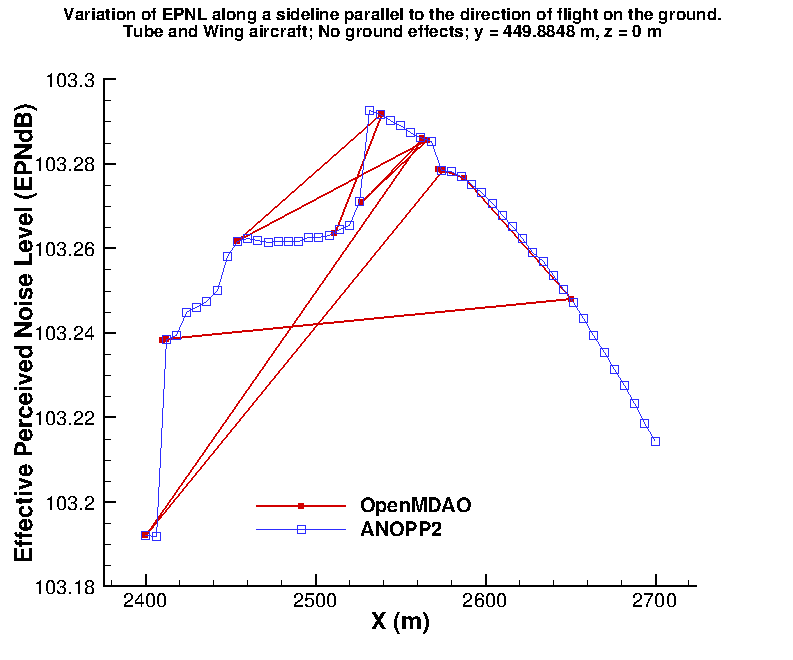
\includegraphics{Optimized.png}
\caption{Variation of EPNL along a sideline showing the sequence of steps followed by OpenMDAO in arriving at the location corresponding to maximum EPNdB}\label{usage:epndb-along-a-sideline}\end{figure}

The observer locations and the corresponding EPNdB values as obtained through \emph{AOIC} are also plotted in {\hyperref[usage:epndb-along-a-sideline]{\emph{EPNdB along a sideline}}} as a sequence of steps (red lines and dots).
The location as found by OpenMDAO that corresponds to maximum EPNdB value along the sideline is at \textbf{2538.5m}.


\chapter{Source Documentation}
\label{srcdocs:anopp2-src-label}\label{srcdocs::doc}\label{srcdocs:source-documentation}
\index{AOIC.py}
The source code \emph{AOIC.py} that uses ANOPP2 routines to identify the location along the sideline of maximum noise is provided as {\hyperref[srcdocs:aoic-py]{\emph{AOIC.py}}}.


\section{AOIC.py}
\label{srcdocs:aoic-py}
\begin{Verbatim}[commandchars=\\\{\},numbers=left,firstnumber=1,stepnumber=1]
\PYG{n}{\PYGZus{}\PYGZus{}all\PYGZus{}\PYGZus{}} \PYG{o}{=} \PYG{p}{[}\PYG{l+s}{\PYGZsq{}}\PYG{l+s}{Anopp2}\PYG{l+s}{\PYGZsq{}}\PYG{p}{]}

\PYG{c}{\PYGZsh{} Import the Component class from the OpenMDAO Main API.}
\PYG{k+kn}{from} \PYG{n+nn}{openmdao.main.api} \PYG{k+kn}{import} \PYG{n}{Component}

\PYG{c}{\PYGZsh{} Import Float class from the Datatypes library in OpenMDAO.}
\PYG{k+kn}{from} \PYG{n+nn}{openmdao.lib.datatypes.api} \PYG{k+kn}{import} \PYG{n}{Float}

\PYG{c}{\PYGZsh{} Import the OpenMDAO library components. We need to import the External Code.}
\PYG{k+kn}{from} \PYG{n+nn}{openmdao.lib.components.external\PYGZus{}code} \PYG{k+kn}{import} \PYG{n}{ExternalCode}

\PYG{c}{\PYGZsh{} Import the FileParser and InputFileGeneration functions residing in Filewrap utility}
\PYG{c}{\PYGZsh{} in OpenMDAO}
\PYG{k+kn}{from} \PYG{n+nn}{openmdao.util.filewrap} \PYG{k+kn}{import} \PYG{n}{FileParser}\PYG{p}{,} \PYG{n}{InputFileGenerator}

\PYG{c}{\PYGZsh{} Import the Float datatype defined in OpenMDAO library required in AOIC.}
\PYG{k+kn}{from} \PYG{n+nn}{openmdao.lib.datatypes.api} \PYG{k+kn}{import} \PYG{n}{Float}

\PYG{c}{\PYGZsh{} Import Numpy as np}
\PYG{k+kn}{import} \PYG{n+nn}{numpy} \PYG{k+kn}{as} \PYG{n+nn}{np}

\PYG{c}{\PYGZsh{} Import the ANOPP2 API python interface.}
\PYG{k+kn}{from} \PYG{n+nn}{ANOPP2\PYGZus{}api} \PYG{k+kn}{import} \PYG{o}{*}

\PYG{c}{\PYGZsh{} Import the ctypes.}
\PYG{k+kn}{from} \PYG{n+nn}{ctypes} \PYG{k+kn}{import} \PYG{o}{*}

\PYG{c}{\PYGZsh{} Import the OS.}
\PYG{k+kn}{import} \PYG{n+nn}{os}

\PYG{k+kn}{from} \PYG{n+nn}{openmdao.main.api} \PYG{k+kn}{import} \PYG{n}{Assembly}
\PYG{c}{\PYGZsh{}from openmdao.lib.drivers.api import SLSQPdriver}

\PYG{c}{\PYGZsh{} Import the Constrained Optimizer driver from the OpenMDAO Optimizers library.}
\PYG{k+kn}{from} \PYG{n+nn}{openmdao.lib.drivers.api} \PYG{k+kn}{import} \PYG{n}{CONMINdriver}



\PYG{c}{\PYGZsh{}====================================================================================}
\PYG{c}{\PYGZsh{} This is the Anopp2Component class that receives the External code. This class is }
\PYG{c}{\PYGZsh{} the crux of AOIC. This uses ANOPP2 function calls to perform various tasks for }
\PYG{c}{\PYGZsh{} predicting noise.  Details of these functions, their syntax, purpose, and usage are}
\PYG{c}{\PYGZsh{} explained in several ANOPP2 Manuals.  Users of ANOPP2 in OpenMDAO are required to}
\PYG{c}{\PYGZsh{} develop this Anopp2Component specific to their problem. }
\PYG{c}{\PYGZsh{}}
\PYG{c}{\PYGZsh{} In this problem, the location of the Observer along a sideline parallel to the}
\PYG{c}{\PYGZsh{} aircraft takeoff on the ground was determined at which the noise (Effective }
\PYG{c}{\PYGZsh{} Perceived Noise Levels (EPNL)) is maximum. This determination is made using }
\PYG{c}{\PYGZsh{} OpenMDAO by minimizing the reciprocal of the EPNL.}
\PYG{c}{\PYGZsh{}====================================================================================}
\PYG{k}{class} \PYG{n+nc}{Anopp2Component}\PYG{p}{(}\PYG{n}{ExternalCode}\PYG{p}{)}\PYG{p}{:}
  \PYG{l+s+sd}{\PYGZdq{}\PYGZdq{}\PYGZdq{}}
\PYG{l+s+sd}{  All ANOPP2\PYGZhy{}capable components should be subclasses of Anopp2Component.}
\PYG{l+s+sd}{   }
\PYG{l+s+sd}{  By subclassing Anopp2Component, any component should have easy access to ANOPP2\PYGZsq{}s}
\PYG{l+s+sd}{  subcomponents, such as Observer, FlightPath, etc.}
\PYG{l+s+sd}{  Refer to Documentation under Anopp2Component for additional information.}
\PYG{l+s+sd}{  \PYGZdq{}\PYGZdq{}\PYGZdq{}}

  \PYG{c}{\PYGZsh{} This is the starting x location of the observer along the sideline, in terms of }
  \PYG{c}{\PYGZsh{} meters. This is set as 2,410 m, the origin being the location at which the flight}
  \PYG{c}{\PYGZsh{} originates.}
  \PYG{n}{x} \PYG{o}{=} \PYG{n}{Float}\PYG{p}{(}\PYG{l+m+mf}{2410.0}\PYG{p}{,} \PYG{n}{iotype}\PYG{o}{=}\PYG{l+s}{\PYGZsq{}}\PYG{l+s}{in}\PYG{l+s}{\PYGZsq{}}\PYG{p}{,} \PYG{n}{desc}\PYG{o}{=}\PYG{l+s}{\PYGZsq{}}\PYG{l+s}{The variable along the direction of flight}\PYG{l+s}{\PYGZsq{}}\PYG{p}{)}
  
  \PYG{c}{\PYGZsh{} This is the inverse of the EpndB. This is the variable that will be optimized or}
  \PYG{c}{\PYGZsh{} minimized.  This variable will be returned by this class.}
  \PYG{n}{Epndb\PYGZus{}inverse} \PYG{o}{=} \PYG{n}{Float}\PYG{p}{(}\PYG{n}{iotype}\PYG{o}{=}\PYG{l+s}{\PYGZsq{}}\PYG{l+s}{out}\PYG{l+s}{\PYGZsq{}}\PYG{p}{,} \PYG{n}{desc}\PYG{o}{=}\PYG{l+s}{\PYGZsq{}}\PYG{l+s}{The inverse of the EPNdB}\PYG{l+s}{\PYGZsq{}}\PYG{p}{)}

  \PYG{c}{\PYGZsh{} Tags for the Atmosphere and Flight Path Data Structures. Although these Data }
  \PYG{c}{\PYGZsh{} Structures will not be used in this demo, the variables are still required as }
  \PYG{c}{\PYGZsh{} input for the routine that creates the mission.}
  \PYG{n}{intAtmosphereTag} \PYG{o}{=} \PYG{n}{c\PYGZus{}int}\PYG{p}{(}\PYG{l+m+mi}{0}\PYG{p}{)}
  \PYG{n}{intFlightPathTag} \PYG{o}{=} \PYG{n}{c\PYGZus{}int}\PYG{p}{(}\PYG{l+m+mi}{0}\PYG{p}{)}
  
  \PYG{c}{\PYGZsh{}  A tag for the observer, which will hold the noise results parsed from the ANOPP}
  \PYG{c}{\PYGZsh{}  output.}
  \PYG{n}{intObserverTag} \PYG{o}{=} \PYG{n}{c\PYGZus{}int}\PYG{p}{(}\PYG{l+m+mi}{0}\PYG{p}{)}
  
  \PYG{c}{\PYGZsh{} A tag for the Functional Module.  For this demonstration program the Funtional }
  \PYG{c}{\PYGZsh{} Module AnoppComplete will be used. A tag name must be declared as follows. This }
  \PYG{c}{\PYGZsh{} tag is set by the a2py\PYGZus{}exec\PYGZus{}create\PYGZus{}functional\PYGZus{}module routine call.}
  \PYG{n}{intAnoppCompleteTag} \PYG{o}{=} \PYG{n}{c\PYGZus{}int}\PYG{p}{(}\PYG{l+m+mi}{0}\PYG{p}{)}
  
  \PYG{c}{\PYGZsh{} This is the number of input Data Structure tags that are required for the }
  \PYG{c}{\PYGZsh{} Functional Module.  In this case, for the AnoppComplete Functional Module there }
  \PYG{c}{\PYGZsh{} will be 0 inputs.}
  \PYG{n}{nInputs} \PYG{o}{=} \PYG{l+m+mi}{0}
  
  \PYG{c}{\PYGZsh{} This is the array of input Data Structure tags, which again, will be of size 0.}
  \PYG{n}{intInputTags} \PYG{o}{=} \PYG{p}{(}\PYG{n}{c\PYGZus{}int} \PYG{o}{*} \PYG{n}{nInputs}\PYG{p}{)}\PYG{p}{(}\PYG{p}{)}
  
  \PYG{c}{\PYGZsh{} This is the number of results from the Functional Module stored in the Observer.}
  \PYG{n}{nResults} \PYG{o}{=} \PYG{n}{c\PYGZus{}int}\PYG{p}{(}\PYG{l+m+mi}{0}\PYG{p}{)}

  \PYG{c}{\PYGZsh{} An array of tags used to access the results in the Observer Data Structure. A }
  \PYG{c}{\PYGZsh{} pointer to this array is returned by the AnoppComplete Functional module.}
  \PYG{n}{intResultTags} \PYG{o}{=} \PYG{n}{pointer}\PYG{p}{(}\PYG{n}{c\PYGZus{}int}\PYG{p}{(}\PYG{l+m+mi}{0}\PYG{p}{)}\PYG{p}{)}

  \PYG{c}{\PYGZsh{} \PYGZhy{}\PYGZhy{}\PYGZhy{}\PYGZhy{}\PYGZhy{}\PYGZhy{}\PYGZhy{}\PYGZhy{}\PYGZhy{}\PYGZhy{}\PYGZhy{}\PYGZhy{}\PYGZhy{}\PYGZhy{}\PYGZhy{}\PYGZhy{}\PYGZhy{}\PYGZhy{}\PYGZhy{}\PYGZhy{}\PYGZhy{}\PYGZhy{}\PYGZhy{}\PYGZhy{}\PYGZhy{}\PYGZhy{}\PYGZhy{}\PYGZhy{}\PYGZhy{}\PYGZhy{}\PYGZhy{}\PYGZhy{}\PYGZhy{}\PYGZhy{}\PYGZhy{}\PYGZhy{}\PYGZhy{}\PYGZhy{}\PYGZhy{}\PYGZhy{}\PYGZhy{}\PYGZhy{}\PYGZhy{}\PYGZhy{}\PYGZhy{}\PYGZhy{}\PYGZhy{}\PYGZhy{}\PYGZhy{}\PYGZhy{}\PYGZhy{}\PYGZhy{}\PYGZhy{}\PYGZhy{}\PYGZhy{}\PYGZhy{}\PYGZhy{}\PYGZhy{}\PYGZhy{}\PYGZhy{}\PYGZhy{}\PYGZhy{}\PYGZhy{}\PYGZhy{}\PYGZhy{}\PYGZhy{}\PYGZhy{}\PYGZhy{}\PYGZhy{}\PYGZhy{}\PYGZhy{}\PYGZhy{}\PYGZhy{}\PYGZhy{}\PYGZhy{}\PYGZhy{}\PYGZhy{}\PYGZhy{}\PYGZhy{}\PYGZhy{}\PYGZhy{}\PYGZhy{}}
  \PYG{c}{\PYGZsh{} Integers and arrays for holding the Functional Module tags and passing them into }
  \PYG{c}{\PYGZsh{} the Mission.  ANOPP2 has 2 types of Functional Modules: \PYGZsq{}Time Series\PYGZsq{} or \PYGZsq{}Single }
  \PYG{c}{\PYGZsh{} Time\PYGZsq{}. The AnoppComplete Functional Module is of type \PYGZsq{}Time Series\PYGZsq{}. Even if a }
  \PYG{c}{\PYGZsh{} user is only utilizing one type of Functional Module, the definitions for arrays }
  \PYG{c}{\PYGZsh{} and parameters need to be provided to the mission for both types.}
  \PYG{c}{\PYGZsh{}\PYGZhy{}\PYGZhy{}\PYGZhy{}\PYGZhy{}\PYGZhy{}\PYGZhy{}\PYGZhy{}\PYGZhy{}\PYGZhy{}\PYGZhy{}\PYGZhy{}\PYGZhy{}\PYGZhy{}\PYGZhy{}\PYGZhy{}\PYGZhy{}\PYGZhy{}\PYGZhy{}\PYGZhy{}\PYGZhy{}\PYGZhy{}\PYGZhy{}\PYGZhy{}\PYGZhy{}\PYGZhy{}\PYGZhy{}\PYGZhy{}\PYGZhy{}\PYGZhy{}\PYGZhy{}\PYGZhy{}\PYGZhy{}\PYGZhy{}\PYGZhy{}\PYGZhy{}\PYGZhy{}\PYGZhy{}\PYGZhy{}\PYGZhy{}\PYGZhy{}\PYGZhy{}\PYGZhy{}\PYGZhy{}\PYGZhy{}\PYGZhy{}\PYGZhy{}\PYGZhy{}\PYGZhy{}\PYGZhy{}\PYGZhy{}\PYGZhy{}\PYGZhy{}\PYGZhy{}\PYGZhy{}\PYGZhy{}\PYGZhy{}\PYGZhy{}\PYGZhy{}\PYGZhy{}\PYGZhy{}\PYGZhy{}\PYGZhy{}\PYGZhy{}\PYGZhy{}\PYGZhy{}\PYGZhy{}\PYGZhy{}\PYGZhy{}\PYGZhy{}\PYGZhy{}\PYGZhy{}\PYGZhy{}\PYGZhy{}\PYGZhy{}\PYGZhy{}\PYGZhy{}\PYGZhy{}\PYGZhy{}\PYGZhy{}\PYGZhy{}\PYGZhy{}\PYGZhy{}\PYGZhy{}}

  \PYG{c}{\PYGZsh{} A tag for the mission, which defines which Function Modules are executed.}
  \PYG{n}{intMissionTag} \PYG{o}{=} \PYG{n}{c\PYGZus{}int}\PYG{p}{(}\PYG{l+m+mi}{0}\PYG{p}{)}

  \PYG{c}{\PYGZsh{} The number of Time Series Functional Modules to be called in the mission.}
  \PYG{c}{\PYGZsh{} For this demonstration there will be 1 (AnoppComplete Functional Module)}
  \PYG{n}{nTimeSeriesFunctionalModules} \PYG{o}{=} \PYG{l+m+mi}{1}

  \PYG{c}{\PYGZsh{} The array of Time Series functional module tags.  This is allocated to size 1}
  \PYG{c}{\PYGZsh{} because there is 1 Time Series Functional Module in this prediction: the }
  \PYG{c}{\PYGZsh{} AnoppComplete Functional Module.}
  \PYG{n}{intTimeSeriesFunctionalModulesTags} \PYG{o}{=} \PYG{p}{(}\PYG{n}{c\PYGZus{}int} \PYG{o}{*} \PYG{n}{nTimeSeriesFunctionalModules}\PYG{p}{)}\PYG{p}{(}\PYG{p}{)}

  \PYG{c}{\PYGZsh{} Single Time definitions are set because the routine to create the mission requires}
  \PYG{c}{\PYGZsh{} these arguments. This demonstration does not have any Single Time Functional }
  \PYG{c}{\PYGZsh{} Modules, therefore all these are set to null or zero values.}

  \PYG{c}{\PYGZsh{} The number of source times for the Single Time Functional Module (time in the }
  \PYG{c}{\PYGZsh{} mission when specific functional modules are executed).  Since there is only a }
  \PYG{c}{\PYGZsh{} Time Series Functional Module, this is not used and is set to 0.}
  \PYG{n}{nSourceTimes} \PYG{o}{=} \PYG{l+m+mi}{0}

  \PYG{c}{\PYGZsh{} The maximum number of Single Time Functional Modules executed at a single source }
  \PYG{c}{\PYGZsh{} time. Since there are no Single Time Functional Modules defined in this }
  \PYG{c}{\PYGZsh{} demonstration, this is set to zero.}
  \PYG{n}{nMaximumSingleTimeFunctionalModules} \PYG{o}{=} \PYG{l+m+mi}{0}

  \PYG{c}{\PYGZsh{} A 2\PYGZhy{}dimensional array of Single Time Functional Module tags.  The first dimension }
  \PYG{c}{\PYGZsh{} is equal to the number of source times, the second is equal to the max number of }
  \PYG{c}{\PYGZsh{} Functional Modules executed per source time.  These are both zero since this }
  \PYG{c}{\PYGZsh{} demonstration does not have any Single Time Functional Modules}
  \PYG{n}{intSingleTimeFunctionalModuleTags} \PYG{o}{=} \PYG{n}{pointer}\PYG{p}{(}\PYG{n}{c\PYGZus{}int}\PYG{p}{(}\PYG{l+m+mi}{0}\PYG{p}{)}\PYG{p}{)}

  \PYG{c}{\PYGZsh{} An array to store the source times.  These can be retrieved from the Flight Path }
  \PYG{c}{\PYGZsh{} API after the Flight Path is created.  However, since there are no Single Time}
  \PYG{c}{\PYGZsh{} Functional Modules, this is allocated to size zero (nSourceTimes is 0).}
  \PYG{n}{fltSourceTimes} \PYG{o}{=} \PYG{n}{pointer}\PYG{p}{(}\PYG{n}{c\PYGZus{}float}\PYG{p}{(}\PYG{l+m+mi}{0}\PYG{p}{)}\PYG{p}{)}

  \PYG{c}{\PYGZsh{} \PYGZhy{}\PYGZhy{}\PYGZhy{}\PYGZhy{}\PYGZhy{}\PYGZhy{}\PYGZhy{}\PYGZhy{}\PYGZhy{}\PYGZhy{}\PYGZhy{}\PYGZhy{}\PYGZhy{}\PYGZhy{}\PYGZhy{}\PYGZhy{}\PYGZhy{}\PYGZhy{}\PYGZhy{}\PYGZhy{}\PYGZhy{}\PYGZhy{}\PYGZhy{}\PYGZhy{}\PYGZhy{}\PYGZhy{}\PYGZhy{}\PYGZhy{}\PYGZhy{}\PYGZhy{}\PYGZhy{}\PYGZhy{}\PYGZhy{}\PYGZhy{}\PYGZhy{}\PYGZhy{}\PYGZhy{}\PYGZhy{}\PYGZhy{}\PYGZhy{}\PYGZhy{}\PYGZhy{}\PYGZhy{}\PYGZhy{}\PYGZhy{}\PYGZhy{}\PYGZhy{}\PYGZhy{}\PYGZhy{}\PYGZhy{}\PYGZhy{}\PYGZhy{}\PYGZhy{}\PYGZhy{}\PYGZhy{}\PYGZhy{}\PYGZhy{}\PYGZhy{}\PYGZhy{}\PYGZhy{}\PYGZhy{}\PYGZhy{}\PYGZhy{}\PYGZhy{}\PYGZhy{}\PYGZhy{}\PYGZhy{}\PYGZhy{}\PYGZhy{}\PYGZhy{}\PYGZhy{}\PYGZhy{}\PYGZhy{}\PYGZhy{}\PYGZhy{}\PYGZhy{}\PYGZhy{}\PYGZhy{}\PYGZhy{}\PYGZhy{}\PYGZhy{}\PYGZhy{}}
  \PYG{c}{\PYGZsh{} An integer success value.  This integer is returned from ANOPP2 API routine calls }
  \PYG{c}{\PYGZsh{} to communicate the state of a given operation.  A return of 0 means success, }
  \PYG{c}{\PYGZsh{} anything other than 0 indicates failure. Note the code execution does not depend }
  \PYG{c}{\PYGZsh{} on this value, hence it is left to the user to check for success and take }
  \PYG{c}{\PYGZsh{} appropriate action.}
  \PYG{c}{\PYGZsh{} \PYGZhy{}\PYGZhy{}\PYGZhy{}\PYGZhy{}\PYGZhy{}\PYGZhy{}\PYGZhy{}\PYGZhy{}\PYGZhy{}\PYGZhy{}\PYGZhy{}\PYGZhy{}\PYGZhy{}\PYGZhy{}\PYGZhy{}\PYGZhy{}\PYGZhy{}\PYGZhy{}\PYGZhy{}\PYGZhy{}\PYGZhy{}\PYGZhy{}\PYGZhy{}\PYGZhy{}\PYGZhy{}\PYGZhy{}\PYGZhy{}\PYGZhy{}\PYGZhy{}\PYGZhy{}\PYGZhy{}\PYGZhy{}\PYGZhy{}\PYGZhy{}\PYGZhy{}\PYGZhy{}\PYGZhy{}\PYGZhy{}\PYGZhy{}\PYGZhy{}\PYGZhy{}\PYGZhy{}\PYGZhy{}\PYGZhy{}\PYGZhy{}\PYGZhy{}\PYGZhy{}\PYGZhy{}\PYGZhy{}\PYGZhy{}\PYGZhy{}\PYGZhy{}\PYGZhy{}\PYGZhy{}\PYGZhy{}\PYGZhy{}\PYGZhy{}\PYGZhy{}\PYGZhy{}\PYGZhy{}\PYGZhy{}\PYGZhy{}\PYGZhy{}\PYGZhy{}\PYGZhy{}\PYGZhy{}\PYGZhy{}\PYGZhy{}\PYGZhy{}\PYGZhy{}\PYGZhy{}\PYGZhy{}\PYGZhy{}\PYGZhy{}\PYGZhy{}\PYGZhy{}\PYGZhy{}\PYGZhy{}\PYGZhy{}\PYGZhy{}\PYGZhy{}\PYGZhy{}}
  \PYG{n}{intSuccess} \PYG{o}{=} \PYG{n}{c\PYGZus{}int}\PYG{p}{(}\PYG{l+m+mi}{0}\PYG{p}{)}
    
  \PYG{c}{\PYGZsh{} This is the number of nodes existing in the Observer.}
  \PYG{n}{nNodes} \PYG{o}{=} \PYG{n}{c\PYGZus{}int}\PYG{p}{(}\PYG{l+m+mi}{0}\PYG{p}{)}

  \PYG{c}{\PYGZsh{} This is the Epnl corresponding to this node.}
  \PYG{n}{fltEpnl} \PYG{o}{=} \PYG{n}{c\PYGZus{}float}\PYG{p}{(}\PYG{o}{\PYGZhy{}}\PYG{l+m+mf}{300.0}\PYG{p}{)}
  
  \PYG{c}{\PYGZsh{} This is the Duration factor determined while calculating EPNL.}
  \PYG{n}{fltD} \PYG{o}{=} \PYG{n}{c\PYGZus{}float}\PYG{p}{(}\PYG{l+m+mi}{0}\PYG{p}{)}
  
  \PYG{c}{\PYGZsh{} This is the minimum and maximum time of the EPNL integration.}
  \PYG{n}{fltTimeRange} \PYG{o}{=} \PYG{p}{(}\PYG{n}{c\PYGZus{}float} \PYG{o}{*} \PYG{l+m+mi}{2}\PYG{p}{)}\PYG{p}{(}\PYG{o}{*}\PYG{p}{[}\PYG{l+m+mf}{0.0}\PYG{p}{,} \PYG{l+m+mf}{0.0}\PYG{p}{]}\PYG{p}{)}
  
  \PYG{c}{\PYGZsh{} This is an array of the position of the last node in the Observer Point Cloud.}
  \PYG{n}{fltPosition} \PYG{o}{=} \PYG{p}{(}\PYG{n}{c\PYGZus{}float} \PYG{o}{*} \PYG{l+m+mi}{3}\PYG{p}{)}\PYG{p}{(}\PYG{o}{*}\PYG{p}{[}\PYG{l+m+mf}{0.0}\PYG{p}{,} \PYG{l+m+mf}{0.0}\PYG{p}{,} \PYG{l+m+mf}{0.0}\PYG{p}{]}\PYG{p}{)}
  

    
  \PYG{c}{\PYGZsh{}===================================================================================}
  \PYG{c}{\PYGZsh{} The Anopp2Component is initialized in this function. Several local variables are }
  \PYG{c}{\PYGZsh{} also initialized. An Observer is created based on the details provided in }
  \PYG{c}{\PYGZsh{} observer.config. }
  \PYG{c}{\PYGZsh{}===================================================================================}
  \PYG{k}{def} \PYG{n+nf}{\PYGZus{}\PYGZus{}init\PYGZus{}\PYGZus{}} \PYG{p}{(}\PYG{n+nb+bp}{self}\PYG{p}{)}\PYG{p}{:}
    \PYG{l+s+sd}{\PYGZdq{}\PYGZdq{}\PYGZdq{} Initialize the Anopp2 class.}
\PYG{l+s+sd}{    \PYGZdq{}\PYGZdq{}\PYGZdq{}}
    \PYG{n+nb}{super}\PYG{p}{(}\PYG{n}{Anopp2Component}\PYG{p}{,} \PYG{n+nb+bp}{self}\PYG{p}{)}\PYG{o}{.}\PYG{n}{\PYGZus{}\PYGZus{}init\PYGZus{}\PYGZus{}}\PYG{p}{(}\PYG{p}{)}

    \PYG{c}{\PYGZsh{}=================================================================================}
    \PYG{c}{\PYGZsh{} Step 1.}
    \PYG{c}{\PYGZsh{} The ANOPP2 API must be initialized before any of the routines can be executed }
    \PYG{c}{\PYGZsh{} and should have false as it\PYGZsq{}s argument.}
    \PYG{c}{\PYGZsh{}=================================================================================}
    \PYG{n}{ANOPP2}\PYG{o}{.}\PYG{n}{a2py\PYGZus{}exec\PYGZus{}init\PYGZus{}api} \PYG{p}{(}\PYG{p}{)}

    \PYG{c}{\PYGZsh{}=================================================================================}
    \PYG{c}{\PYGZsh{} Step 2.}
    \PYG{c}{\PYGZsh{} Create the necessary Data Structures required by the Anopp Complete Functional }
    \PYG{c}{\PYGZsh{} Module. Set the tag numbers to zero for the Data Structures that ANOPP will }
    \PYG{c}{\PYGZsh{} generate internally when it is executed.  This are necessary becuase the }
    \PYG{c}{\PYGZsh{} variables are requried in the definition of the routine that creates the }
    \PYG{c}{\PYGZsh{} mission. The Observer must be given to the Functional Module, so it must be }
    \PYG{c}{\PYGZsh{} created from a configuration file.}
    \PYG{c}{\PYGZsh{}=================================================================================}
    \PYG{n+nb+bp}{self}\PYG{o}{.}\PYG{n}{intAtmosphereTag} \PYG{o}{=} \PYG{l+m+mi}{0}
    \PYG{n+nb+bp}{self}\PYG{o}{.}\PYG{n}{intFlightPathTag} \PYG{o}{=} \PYG{l+m+mi}{0}

    \PYG{c}{\PYGZsh{}=================================================================================}
    \PYG{c}{\PYGZsh{} Step 3.}
    \PYG{c}{\PYGZsh{} Construct an observer point (only a single point is used for serial execution) }
    \PYG{c}{\PYGZsh{} from a configuration file.  This is done by using the create function of the }
    \PYG{c}{\PYGZsh{} Observer API and passing a blank observer tag and the file name.  The necessary}
    \PYG{c}{\PYGZsh{}  configuration file accompanies this demonstrator..}
    \PYG{c}{\PYGZsh{}=================================================================================}
    \PYG{n}{intSuccess} \PYG{o}{=}             \PYGZbs{}
      \PYG{n}{ANOPP2}\PYG{o}{.}\PYG{n}{a2py\PYGZus{}obs\PYGZus{}create} \PYGZbs{}
       \PYG{p}{(}\PYG{n}{pointer}\PYG{p}{(}\PYG{n+nb+bp}{self}\PYG{o}{.}\PYG{n}{intObserverTag}\PYG{p}{)}\PYG{p}{,} \PYG{n}{create\PYGZus{}string\PYGZus{}buffer} \PYG{p}{(}\PYG{n}{b}\PYG{l+s}{\PYGZdq{}}\PYG{l+s}{observer.config}\PYG{l+s}{\PYGZdq{}}\PYG{p}{)}\PYG{p}{)}



  \PYG{c}{\PYGZsh{}===================================================================================}
  \PYG{c}{\PYGZsh{} The execute function gets executed by OpenMDAO repeatedly until the specified}
  \PYG{c}{\PYGZsh{} exit criteria are met. The steps followed in this function are:}
  \PYG{c}{\PYGZsh{}   1. Obtain the number of nodes available in the observer.}
  \PYG{c}{\PYGZsh{}   2. Obtain the position vector of the lsat node in the observer.}
  \PYG{c}{\PYGZsh{}   3. Replace the x\PYGZhy{}coordinate of this position vector with that provided by the}
  \PYG{c}{\PYGZsh{}      OpenMDAO optimizer.}
  \PYG{c}{\PYGZsh{}   4. Insert a new node in the observer with a position vector as defined through}
  \PYG{c}{\PYGZsh{}      steps 2 through 4.}
  \PYG{c}{\PYGZsh{}   5. Create an AnoppComplete Functional Module based on the config file,}
  \PYG{c}{\PYGZsh{}      \PYGZdq{}AnoppComplete.config\PYGZdq{}.}
  \PYG{c}{\PYGZsh{}   6. Create a mission for running AnoppComplete functional module and executing }
  \PYG{c}{\PYGZsh{}      ANOPP to obtain noise due to Jet, Inlet, Aft Fan, Core, Gear, Flap, and }
  \PYG{c}{\PYGZsh{}      Trailing edge are all added to obtain the total noise. This noise is then}
  \PYG{c}{\PYGZsh{}      propagated to the ground observer.}
  \PYG{c}{\PYGZsh{}   7. Execute the mission to obtain the total noise on the ground observer.}
  \PYG{c}{\PYGZsh{}   8. Obtain the number of results in the Observer.}
  \PYG{c}{\PYGZsh{}   9. Obtain the number of nodes in the Observer.}
  \PYG{c}{\PYGZsh{}  10. Calculate the EPNL from the acoustic data predicted by the AnoppComplete}
  \PYG{c}{\PYGZsh{}      functional module.}
  \PYG{c}{\PYGZsh{}  11. Get the EPNL value of the last node.}
  \PYG{c}{\PYGZsh{}  12. If the EPNL value is valid, get its inverse. The inverse of the EPNL is }
  \PYG{c}{\PYGZsh{}      numerically small. Multiply it with 1000 and treat this as EpndB\PYGZus{}inverse.}
  \PYG{c}{\PYGZsh{}  13. Export the results to a Tecplot\PYGZhy{}friendly file.}
  \PYG{c}{\PYGZsh{}  14. Delete the results because we do not need it any more.}
  \PYG{c}{\PYGZsh{}===================================================================================}
  \PYG{k}{def} \PYG{n+nf}{execute}\PYG{p}{(}\PYG{n+nb+bp}{self}\PYG{p}{)}\PYG{p}{:}
    \PYG{l+s+sd}{\PYGZdq{}\PYGZdq{}\PYGZdq{} Obtain a given Observer location, find the noise at that location. Use such }
\PYG{l+s+sd}{    noise values to optimize and locate the Observer location that has the maximum }
\PYG{l+s+sd}{    noise.}
\PYG{l+s+sd}{    \PYGZdq{}\PYGZdq{}\PYGZdq{}}
       
    \PYG{c}{\PYGZsh{}=================================================================================}
    \PYG{c}{\PYGZsh{} Step 4. We need to introduce a new node at a location provided by the optimizer.}
    \PYG{c}{\PYGZsh{} To do that, we need to first find the location of the last node in the observer, }
    \PYG{c}{\PYGZsh{} replace the x coordinate of this node location with that provided by the }
    \PYG{c}{\PYGZsh{} optimizer, and then introduce it as a new node in the point cloud.}
    \PYG{c}{\PYGZsh{}=================================================================================}

    \PYG{c}{\PYGZsh{} Get the number of nodes in the Observer.}
    \PYG{n}{intSuccess} \PYG{o}{=} \PYG{n}{ANOPP2}\PYG{o}{.}\PYG{n}{a2py\PYGZus{}obs\PYGZus{}number\PYGZus{}of\PYGZus{}nodes} \PYG{p}{(}\PYG{n+nb+bp}{self}\PYG{o}{.}\PYG{n}{intObserverTag}\PYG{p}{,} \PYG{n+nb+bp}{self}\PYG{o}{.}\PYG{n}{nNodes}\PYG{p}{)}
    
    \PYG{c}{\PYGZsh{} Get the coordinates of the last node.}
    \PYG{n}{intSuccess} \PYG{o}{=}               \PYGZbs{}
      \PYG{n}{ANOPP2}\PYG{o}{.}\PYG{n}{a2py\PYGZus{}obs\PYGZus{}position} \PYGZbs{}
        \PYG{p}{(}\PYG{n+nb+bp}{self}\PYG{o}{.}\PYG{n}{intObserverTag}\PYG{p}{,} \PYG{n+nb+bp}{self}\PYG{o}{.}\PYG{n}{nNodes}\PYG{p}{,} \PYG{l+m+mf}{0.0}\PYG{p}{,} \PYG{n}{a2\PYGZus{}global}\PYG{p}{,} \PYG{n+nb+bp}{self}\PYG{o}{.}\PYG{n}{fltPosition}\PYG{p}{)}
        
    \PYG{c}{\PYGZsh{} Replace the x coordinates of this array with that from the class. Rest of the }
    \PYG{c}{\PYGZsh{} coordinates remain the same.}
    \PYG{n+nb+bp}{self}\PYG{o}{.}\PYG{n}{fltPosition}\PYG{p}{[}\PYG{l+m+mi}{0}\PYG{p}{]} \PYG{o}{=} \PYG{n+nb+bp}{self}\PYG{o}{.}\PYG{n}{x}
    
    \PYG{c}{\PYGZsh{} Insert a new node to the Point Cloud in the Observer.}
    \PYG{n}{intSuccess} \PYG{o}{=} \PYG{n}{ANOPP2}\PYG{o}{.}\PYG{n}{a2py\PYGZus{}obs\PYGZus{}new\PYGZus{}node} \PYG{p}{(}\PYG{n+nb+bp}{self}\PYG{o}{.}\PYG{n}{intObserverTag}\PYG{p}{,} \PYG{n+nb+bp}{self}\PYG{o}{.}\PYG{n}{fltPosition}\PYG{p}{)}

    \PYG{c}{\PYGZsh{}=================================================================================}
    \PYG{c}{\PYGZsh{} Step 5.}
    \PYG{c}{\PYGZsh{} Create the AnoppComplete Functional Module.}
    \PYG{c}{\PYGZsh{}=================================================================================}
    
    \PYG{c}{\PYGZsh{} Create the AnoppComplete Functional Module by passing an empty tag number (to be}
    \PYG{c}{\PYGZsh{} filled), the configuration file name, the number of inputs, the list of Data }
    \PYG{c}{\PYGZsh{} structure Tags, a pointer to the Observer tag, the number of results, and a }
    \PYG{c}{\PYGZsh{} pointer to the array of result tags. The number of results and the result tags }
    \PYG{c}{\PYGZsh{} are returned from the create function and can be used to later access the data }
    \PYG{c}{\PYGZsh{} stored in the Observer Data Structure.}
    \PYG{n}{intSuccess} \PYG{o}{=}                                                                 \PYGZbs{}
      \PYG{n}{ANOPP2}\PYG{o}{.}\PYG{n}{a2py\PYGZus{}exec\PYGZus{}create\PYGZus{}functional\PYGZus{}module}                                  \PYGZbs{}
       \PYG{p}{(}\PYG{n}{pointer}\PYG{p}{(}\PYG{n+nb+bp}{self}\PYG{o}{.}\PYG{n}{intAnoppCompleteTag}\PYG{p}{)}\PYG{p}{,}                                       \PYGZbs{}
        \PYG{n}{create\PYGZus{}string\PYGZus{}buffer} \PYG{p}{(}\PYG{n}{b}\PYG{l+s}{\PYGZdq{}}\PYG{l+s}{AnoppComplete.config}\PYG{l+s}{\PYGZdq{}}\PYG{p}{)}\PYG{p}{,} \PYG{n+nb+bp}{self}\PYG{o}{.}\PYG{n}{nInputs}\PYG{p}{,}            \PYGZbs{}
        \PYG{n+nb+bp}{self}\PYG{o}{.}\PYG{n}{intInputTags}\PYG{p}{,} \PYG{n}{pointer}\PYG{p}{(}\PYG{n+nb+bp}{self}\PYG{o}{.}\PYG{n}{intObserverTag}\PYG{p}{)}\PYG{p}{,} \PYG{n}{pointer}\PYG{p}{(}\PYG{n+nb+bp}{self}\PYG{o}{.}\PYG{n}{nResults}\PYG{p}{)}\PYG{p}{,} \PYGZbs{}
        \PYG{n}{pointer}\PYG{p}{(}\PYG{n+nb+bp}{self}\PYG{o}{.}\PYG{n}{intResultTags}\PYG{p}{)}\PYG{p}{)}

    \PYG{c}{\PYGZsh{}=================================================================================}
    \PYG{c}{\PYGZsh{} Step 6.}
    \PYG{c}{\PYGZsh{} Create the Mission.  The Mission is the definition of what Functional Modules }
    \PYG{c}{\PYGZsh{} will be executed. In this example, only the AnoppComplete Functional Module will}
    \PYG{c}{\PYGZsh{} be executed for all time.}
    \PYG{c}{\PYGZsh{}=================================================================================}

    \PYG{c}{\PYGZsh{} Since the only Time Series Functional Module being used is AnoppComplete, assign}
    \PYG{c}{\PYGZsh{} it to the first and only index of the array (if there was a second Time Series }
    \PYG{c}{\PYGZsh{} Functional Module, it would be assigned to the second index of the array).}
    \PYG{n+nb+bp}{self}\PYG{o}{.}\PYG{n}{intTimeSeriesFunctionalModulesTags} \PYG{p}{[}\PYG{l+m+mi}{0}\PYG{p}{]} \PYG{o}{=} \PYG{n+nb+bp}{self}\PYG{o}{.}\PYG{n}{intAnoppCompleteTag}

    \PYG{c}{\PYGZsh{} To create a mission, each Functional Module tag must be added to the Mission }
    \PYG{c}{\PYGZsh{} according to its type placed in arrays of the appropriate structure.  If Single }
    \PYG{c}{\PYGZsh{} Time Functional Modules exist, then their tags would be placed into a two }
    \PYG{c}{\PYGZsh{} dimensional array corresponding to waypoints and number of Single Time }
    \PYG{c}{\PYGZsh{} Functional Modules. Time Series Functional Modules have their tags placed in a }
    \PYG{c}{\PYGZsh{} one dimensional array. The routine to create a Mission also requires the }
    \PYG{c}{\PYGZsh{} waypoint times, and the Atmosphere and Flight Path tags, regardless of  whether }
    \PYG{c}{\PYGZsh{} they are being used. In this case they are not, so their values are set to zero.}
    \PYG{c}{\PYGZsh{} Note: This demonstration program has only one Functional Module: AnoppComplete. }
    \PYG{c}{\PYGZsh{} This is a Time Series Functional Module and therefore, all Single Time }
    \PYG{c}{\PYGZsh{} Functional Module inputs are left empty.  The only reason they are needed is }
    \PYG{c}{\PYGZsh{} because the a2py\PYGZus{}exec\PYGZus{}create\PYGZus{}mission requires them.}
    \PYG{n}{intSuccess} \PYG{o}{=}                                                                     \PYGZbs{}
      \PYG{n}{ANOPP2}\PYG{o}{.}\PYG{n}{a2py\PYGZus{}exec\PYGZus{}create\PYGZus{}mission}                                                \PYGZbs{}
       \PYG{p}{(}\PYG{n}{pointer}\PYG{p}{(}\PYG{n+nb+bp}{self}\PYG{o}{.}\PYG{n}{intMissionTag}\PYG{p}{)}\PYG{p}{,} \PYG{n}{create\PYGZus{}string\PYGZus{}buffer} \PYG{p}{(}\PYG{n}{b}\PYG{l+s}{\PYGZdq{}}\PYG{l+s}{\PYGZdq{}}\PYG{p}{)}\PYG{p}{,}                     \PYGZbs{}
        \PYG{n+nb+bp}{self}\PYG{o}{.}\PYG{n}{intAtmosphereTag}\PYG{p}{,} \PYG{n+nb+bp}{self}\PYG{o}{.}\PYG{n}{intFlightPathTag}\PYG{p}{,} \PYG{n+nb+bp}{self}\PYG{o}{.}\PYG{n}{nSourceTimes}\PYG{p}{,}             \PYGZbs{}
        \PYG{n+nb+bp}{self}\PYG{o}{.}\PYG{n}{nMaximumSingleTimeFunctionalModules}\PYG{p}{,} \PYG{n+nb+bp}{self}\PYG{o}{.}\PYG{n}{nTimeSeriesFunctionalModules}\PYG{p}{,} \PYGZbs{}
        \PYG{n+nb+bp}{self}\PYG{o}{.}\PYG{n}{fltSourceTimes}\PYG{p}{,} \PYG{n+nb+bp}{self}\PYG{o}{.}\PYG{n}{intSingleTimeFunctionalModuleTags}\PYG{p}{,}                 \PYGZbs{}
        \PYG{n+nb+bp}{self}\PYG{o}{.}\PYG{n}{intTimeSeriesFunctionalModulesTags}\PYG{p}{)}

    \PYG{c}{\PYGZsh{}=================================================================================}
    \PYG{c}{\PYGZsh{} Step 7.}
    \PYG{c}{\PYGZsh{} Execute the Mission.  The Mission performs the noise prediction.  This call }
    \PYG{c}{\PYGZsh{} tells the Mission to execute all Functional Modules at the time specified. This }
    \PYG{c}{\PYGZsh{} will in turn execute ANOPP, producing a fort.4 that will be renamed to the }
    \PYG{c}{\PYGZsh{} output specified in the configuration file}
    \PYG{c}{\PYGZsh{}=================================================================================}

    \PYG{c}{\PYGZsh{}  Call the routine that executes the Mission}
    \PYG{n}{intSuccess} \PYG{o}{=} \PYG{n}{ANOPP2}\PYG{o}{.}\PYG{n}{a2py\PYGZus{}exec\PYGZus{}execute\PYGZus{}mission} \PYG{p}{(}\PYG{n+nb+bp}{self}\PYG{o}{.}\PYG{n}{intMissionTag}\PYG{p}{)}
    
    \PYG{c}{\PYGZsh{} Get the number of results in the Observer.}
    \PYG{n}{intSuccess} \PYG{o}{=} \PYGZbs{}
      \PYG{n}{ANOPP2}\PYG{o}{.}\PYG{n}{a2py\PYGZus{}obs\PYGZus{}number\PYGZus{}of\PYGZus{}results} \PYG{p}{(}\PYG{n+nb+bp}{self}\PYG{o}{.}\PYG{n}{intObserverTag}\PYG{p}{,} \PYG{n+nb+bp}{self}\PYG{o}{.}\PYG{n}{nResults}\PYG{p}{)}

    \PYG{c}{\PYGZsh{}=================================================================================}
    \PYG{c}{\PYGZsh{} Step 8.}
    \PYG{c}{\PYGZsh{} Calculate metrics and report the results. After the Mission is executed, the }
    \PYG{c}{\PYGZsh{} Observer Data Structure contains the prediction results. These results can be }
    \PYG{c}{\PYGZsh{} accessed to calculate derived metrics and reported to an external file using }
    \PYG{c}{\PYGZsh{} Observer API routine calls.  To calculate metrics, the Observer API provides }
    \PYG{c}{\PYGZsh{} specific acoustic analysis functionality that can be invoked via input }
    \PYG{c}{\PYGZsh{} enumerators.  A list of the enumerators available for the Observer API routines }
    \PYG{c}{\PYGZsh{} can be found in the Observer API User\PYGZsq{}s Manual.}
    \PYG{c}{\PYGZsh{}=================================================================================}
       
    \PYG{c}{\PYGZsh{} Get the number of nodes in the Observer.}
    \PYG{n}{intSuccess} \PYG{o}{=} \PYG{n}{ANOPP2}\PYG{o}{.}\PYG{n}{a2py\PYGZus{}obs\PYGZus{}number\PYGZus{}of\PYGZus{}nodes} \PYG{p}{(}\PYG{n+nb+bp}{self}\PYG{o}{.}\PYG{n}{intObserverTag}\PYG{p}{,} \PYG{n+nb+bp}{self}\PYG{o}{.}\PYG{n}{nNodes}\PYG{p}{)}

    \PYG{c}{\PYGZsh{} The first step is to calculate any derived metrics. For this demonstrator, EPNL }
    \PYG{c}{\PYGZsh{} is calculated. The first argument in the call is the observer tag. The second }
    \PYG{c}{\PYGZsh{} argument is the array containing the result tags associated with the observer}
    \PYG{c}{\PYGZsh{} locations.  In this case there are three results, Engine, Airframe, and Total. }
    \PYG{c}{\PYGZsh{} The third argument is an enumerator for what noise metric will be calculated and}
    \PYG{c}{\PYGZsh{} returned by this call. For this demonstration the metric is EPNL. The last }
    \PYG{c}{\PYGZsh{} argument is an enumerator that tells the Observer API that the EPNL has to be\PYGZsq{}}
    \PYG{c}{\PYGZsh{} calculated based on the complete time history.  This is defined by the }
    \PYG{c}{\PYGZsh{} enumerator, a2\PYGZus{}obs\PYGZus{}complete.}
    \PYG{n}{intSuccess} \PYG{o}{=}                                                                  \PYGZbs{}
      \PYG{n}{ANOPP2}\PYG{o}{.}\PYG{n}{a2py\PYGZus{}obs\PYGZus{}calc\PYGZus{}metric}                                                 \PYGZbs{}
       \PYG{p}{(}\PYG{n+nb+bp}{self}\PYG{o}{.}\PYG{n}{intObserverTag}\PYG{p}{,} \PYG{n+nb+bp}{self}\PYG{o}{.}\PYG{n}{nResults}\PYG{o}{.}\PYG{n}{value}\PYG{p}{,} \PYG{n+nb+bp}{self}\PYG{o}{.}\PYG{n}{intResultTags}\PYG{p}{,} \PYG{n}{a2\PYGZus{}aa\PYGZus{}epnl}\PYG{p}{,} \PYGZbs{}
        \PYG{n}{a2\PYGZus{}obs\PYGZus{}complete}\PYG{p}{)}

    \PYG{c}{\PYGZsh{} Get the EPNL value for the last node which is the node that was inserted into }
    \PYG{c}{\PYGZsh{} the Observer.}
    \PYG{n}{intSuccess} \PYG{o}{=}                                                        \PYGZbs{}
      \PYG{n}{ANOPP2}\PYG{o}{.}\PYG{n}{a2py\PYGZus{}obs\PYGZus{}get\PYGZus{}epnl}                                          \PYGZbs{}
        \PYG{p}{(}\PYG{n+nb+bp}{self}\PYG{o}{.}\PYG{n}{intObserverTag}\PYG{p}{,} \PYG{n+nb+bp}{self}\PYG{o}{.}\PYG{n}{intResultTags}\PYG{p}{[}\PYG{l+m+mi}{0}\PYG{p}{]}\PYG{p}{,} \PYG{n+nb+bp}{self}\PYG{o}{.}\PYG{n}{nNodes}\PYG{o}{.}\PYG{n}{value}\PYG{p}{,} \PYGZbs{}
         \PYG{n+nb+bp}{self}\PYG{o}{.}\PYG{n}{fltEpnl}\PYG{p}{,} \PYG{n+nb+bp}{self}\PYG{o}{.}\PYG{n}{fltD}\PYG{p}{,} \PYG{n+nb+bp}{self}\PYG{o}{.}\PYG{n}{fltTimeRange}\PYG{p}{)}
    
    \PYG{c}{\PYGZsh{} Ensure that the EPNL obtained from the Observer is greater than zero and is not }
    \PYG{c}{\PYGZsh{} none.}
    \PYG{k}{if} \PYG{p}{(}\PYG{n+nb+bp}{self}\PYG{o}{.}\PYG{n}{fltEpnl} \PYG{o+ow}{is} \PYG{o+ow}{not} \PYG{n+nb+bp}{None}\PYG{p}{)} \PYG{o+ow}{and} \PYG{p}{(}\PYG{n+nb+bp}{self}\PYG{o}{.}\PYG{n}{fltEpnl}\PYG{o}{.}\PYG{n}{value} \PYG{o}{\PYGZgt{}} \PYG{l+m+mf}{0.0}\PYG{p}{)}\PYG{p}{:}

      \PYG{c}{\PYGZsh{} Set the Epndb inverse as the reciprocal of the Epndb.}
      \PYG{n+nb+bp}{self}\PYG{o}{.}\PYG{n}{Epndb\PYGZus{}inverse} \PYG{o}{=} \PYG{l+m+mf}{1000.0}\PYG{o}{/}\PYG{n+nb}{float}\PYG{p}{(}\PYG{n+nb+bp}{self}\PYG{o}{.}\PYG{n}{fltEpnl}\PYG{o}{.}\PYG{n}{value}\PYG{p}{)}

    \PYG{c}{\PYGZsh{} Print the Location and the EPNL values to the screen.}
    \PYG{k}{print} \PYG{p}{(}\PYG{l+s}{\PYGZdq{}}\PYG{l+s}{Location: }\PYG{l+s}{\PYGZdq{}}\PYG{p}{,} \PYG{n+nb+bp}{self}\PYG{o}{.}\PYG{n}{fltPosition}\PYG{p}{[}\PYG{l+m+mi}{0}\PYG{p}{]}\PYG{p}{)}
    \PYG{k}{print} \PYG{p}{(}\PYG{l+s}{\PYGZdq{}}\PYG{l+s}{EPNL: }\PYG{l+s}{\PYGZdq{}}\PYG{p}{,} \PYG{n+nb+bp}{self}\PYG{o}{.}\PYG{n}{fltEpnl}\PYG{o}{.}\PYG{n}{value}\PYG{p}{)}
    
    \PYG{c}{\PYGZsh{} Set the Output file name for exporting the EPNL to a file.}
    \PYG{n+nb+bp}{self}\PYG{o}{.}\PYG{n}{strOutputFile} \PYG{o}{=} \PYG{l+s}{\PYGZdq{}}\PYG{l+s}{Epnl.out.dat}\PYG{l+s}{\PYGZdq{}}
    
    \PYG{c}{\PYGZsh{} Export the result to a file.}
    \PYG{n}{intSuccess} \PYG{o}{=}                                                                 \PYGZbs{}
      \PYG{n}{ANOPP2}\PYG{o}{.}\PYG{n}{a2py\PYGZus{}obs\PYGZus{}export}                                                     \PYGZbs{}
        \PYG{p}{(}\PYG{n+nb+bp}{self}\PYG{o}{.}\PYG{n}{intObserverTag}\PYG{p}{,} \PYG{n+nb+bp}{self}\PYG{o}{.}\PYG{n}{intResultTags}\PYG{p}{[}\PYG{l+m+mi}{0}\PYG{p}{]}\PYG{p}{,}                             \PYGZbs{}
         \PYG{n}{create\PYGZus{}string\PYGZus{}buffer}\PYG{p}{(}\PYG{n+nb}{bytes}\PYG{p}{(}\PYG{n+nb+bp}{self}\PYG{o}{.}\PYG{n}{strOutputFile}\PYG{p}{)}\PYG{p}{)}\PYG{p}{,} \PYG{n}{a2\PYGZus{}aa\PYGZus{}epnl}\PYG{p}{,} \PYG{n}{a2\PYGZus{}global}\PYG{p}{,} \PYGZbs{}
         \PYG{n}{a2\PYGZus{}formatted}\PYG{p}{,} \PYG{n}{a2\PYGZus{}tecplot}\PYG{p}{)}
    
    \PYG{c}{\PYGZsh{} Delete the results because we don\PYGZsq{}t need them any more.}
    \PYG{n}{intSuccess} \PYG{o}{=}                     \PYGZbs{}
      \PYG{n}{ANOPP2}\PYG{o}{.}\PYG{n}{a2py\PYGZus{}obs\PYGZus{}delete\PYGZus{}results} \PYGZbs{}
        \PYG{p}{(}\PYG{n+nb+bp}{self}\PYG{o}{.}\PYG{n}{intObserverTag}\PYG{p}{,} \PYG{n+nb+bp}{self}\PYG{o}{.}\PYG{n}{nResults}\PYG{o}{.}\PYG{n}{value}\PYG{p}{,} \PYG{n+nb+bp}{self}\PYG{o}{.}\PYG{n}{intResultTags}\PYG{p}{,} \PYG{l+m+mi}{0}\PYG{p}{)}



\PYG{c}{\PYGZsh{}====================================================================================}
\PYG{c}{\PYGZsh{} This class contains the optimizer. It defines the design variable (the variable }
\PYG{c}{\PYGZsh{} that has to be varied) and the parameter to be minimized (Epndb\PYGZus{}inverse) and calls }
\PYG{c}{\PYGZsh{} the Anopp2Component class repeatedly. It also specifies the driver to be used for}
\PYG{c}{\PYGZsh{} optimization and the criteria for optimizing and exiting the optimization.}
\PYG{c}{\PYGZsh{} This class performs the following steps:}
\PYG{c}{\PYGZsh{}   1. It adds the Driver to be used and assigns a name to it. Two drivers have been }
\PYG{c}{\PYGZsh{}      tried out: SLSQPdriver and CONMINdriver.}
\PYG{c}{\PYGZsh{}   2. It adds the Anopp2Component class and assigns a name to it.}
\PYG{c}{\PYGZsh{}   3. It adds this Anopp2Component to the Workflow of the driver.}
\PYG{c}{\PYGZsh{}   4. It specifies the interval to display the optimization details.}
\PYG{c}{\PYGZsh{}   5. It then adds the Objective variable and the parameter variable to be minimed.}
\PYG{c}{\PYGZsh{}   6. Depending on the driver chosen it specifies the set of parameters for }
\PYG{c}{\PYGZsh{}      optimization. }
\PYG{c}{\PYGZsh{}====================================================================================}
\PYG{k}{class} \PYG{n+nc}{Anopp2Optimize}\PYG{p}{(}\PYG{n}{Assembly}\PYG{p}{)}\PYG{p}{:}
  \PYG{l+s+sd}{\PYGZdq{}\PYGZdq{}\PYGZdq{}Unconstrained Optimization to locate the Observer location corresponding to }
\PYG{l+s+sd}{  maximum EpndB\PYGZdq{}\PYGZdq{}\PYGZdq{}}



  \PYG{k}{def} \PYG{n+nf}{configure}\PYG{p}{(}\PYG{n+nb+bp}{self}\PYG{p}{)}\PYG{p}{:}
    
    \PYG{c}{\PYGZsh{} Create an optimizer instance (Uncomment the following statement if SLSQP driver }
    \PYG{c}{\PYGZsh{} is to be used, and comment the next statement.}
\PYG{c}{\PYGZsh{}    self.add(\PYGZsq{}driver\PYGZsq{}, SLSQPdriver())}
    \PYG{n+nb+bp}{self}\PYG{o}{.}\PYG{n}{add}\PYG{p}{(}\PYG{l+s}{\PYGZsq{}}\PYG{l+s}{driver}\PYG{l+s}{\PYGZsq{}}\PYG{p}{,} \PYG{n}{CONMINdriver}\PYG{p}{(}\PYG{p}{)}\PYG{p}{)}
    
    \PYG{c}{\PYGZsh{} Create Anopp2 component instance.}
    \PYG{n+nb+bp}{self}\PYG{o}{.}\PYG{n}{add}\PYG{p}{(}\PYG{l+s}{\PYGZsq{}}\PYG{l+s}{anopp2}\PYG{l+s}{\PYGZsq{}}\PYG{p}{,} \PYG{n}{Anopp2Component}\PYG{p}{(}\PYG{p}{)}\PYG{p}{)}
    
    \PYG{c}{\PYGZsh{} Iteration hierarchy}
    \PYG{n+nb+bp}{self}\PYG{o}{.}\PYG{n}{driver}\PYG{o}{.}\PYG{n}{workflow}\PYG{o}{.}\PYG{n}{add}\PYG{p}{(}\PYG{l+s}{\PYGZsq{}}\PYG{l+s}{anopp2}\PYG{l+s}{\PYGZsq{}}\PYG{p}{)}
    
    \PYG{c}{\PYGZsh{} SLSQP Flags}
    \PYG{n+nb+bp}{self}\PYG{o}{.}\PYG{n}{driver}\PYG{o}{.}\PYG{n}{iprint} \PYG{o}{=} \PYG{l+m+mi}{1}
    
    \PYG{c}{\PYGZsh{} Objective}
    \PYG{n+nb+bp}{self}\PYG{o}{.}\PYG{n}{driver}\PYG{o}{.}\PYG{n}{add\PYGZus{}objective}\PYG{p}{(}\PYG{l+s}{\PYGZsq{}}\PYG{l+s}{anopp2.Epndb\PYGZus{}inverse}\PYG{l+s}{\PYGZsq{}}\PYG{p}{)}
    
    \PYG{c}{\PYGZsh{} Design variable}
    \PYG{n+nb+bp}{self}\PYG{o}{.}\PYG{n}{driver}\PYG{o}{.}\PYG{n}{add\PYGZus{}parameter}\PYG{p}{(}\PYG{l+s}{\PYGZsq{}}\PYG{l+s}{anopp2.x}\PYG{l+s}{\PYGZsq{}}\PYG{p}{,} \PYG{n}{low}\PYG{o}{=}\PYG{l+m+mf}{2400.}\PYG{p}{,} \PYG{n}{high}\PYG{o}{=}\PYG{l+m+mf}{3500.0}\PYG{p}{)}
    
    \PYG{c}{\PYGZsh{} Set the SLSQP\PYGZhy{}specific settings. Uncomment the following if SLSQP Driver is to}
    \PYG{c}{\PYGZsh{} be used.}
\PYG{c}{\PYGZsh{}    self.driver.accuracy = 1.0e\PYGZhy{}08}
\PYG{c}{\PYGZsh{}    self.driver.maxiter = 50}
    
    \PYG{c}{\PYGZsh{} Set the CONMIN\PYGZhy{}specific settings. Comment the following if SLSQP Driver is to be}
    \PYG{c}{\PYGZsh{} used.}
    \PYG{n+nb+bp}{self}\PYG{o}{.}\PYG{n}{driver}\PYG{o}{.}\PYG{n}{itmax} \PYG{o}{=} \PYG{l+m+mi}{30}
    \PYG{n+nb+bp}{self}\PYG{o}{.}\PYG{n}{driver}\PYG{o}{.}\PYG{n}{fdch} \PYG{o}{=} \PYG{l+m+mf}{0.001}
    \PYG{n+nb+bp}{self}\PYG{o}{.}\PYG{n}{driver}\PYG{o}{.}\PYG{n}{fdchm} \PYG{o}{=} \PYG{l+m+mf}{0.0001}
    \PYG{n+nb+bp}{self}\PYG{o}{.}\PYG{n}{driver}\PYG{o}{.}\PYG{n}{ctlmin} \PYG{o}{=} \PYG{l+m+mf}{0.01}
    \PYG{n+nb+bp}{self}\PYG{o}{.}\PYG{n}{driver}\PYG{o}{.}\PYG{n}{delfun} \PYG{o}{=} \PYG{l+m+mf}{0.01}
    \PYG{n+nb+bp}{self}\PYG{o}{.}\PYG{n}{driver}\PYG{o}{.}\PYG{n}{conmin\PYGZus{}diff} \PYG{o}{=} \PYG{n+nb+bp}{True}
    \PYG{n+nb+bp}{self}\PYG{o}{.}\PYG{n}{iIteration} \PYG{o}{=} \PYG{l+m+mi}{0}
\end{Verbatim}

The code for testing this \emph{AOIC.py} is provided as {\hyperref[srcdocs:test-aoic-py]{\emph{test\_aoic.py}}}.


\section{test\_aoic.py}
\label{srcdocs:test-aoic-py}
\begin{Verbatim}[commandchars=\\\{\},numbers=left,firstnumber=1,stepnumber=1]
\PYG{c}{\PYGZsh{}====================================================================================}
\PYG{c}{\PYGZsh{} This program is a unit test that tests the Anopp2 optimization problem.}
\PYG{c}{\PYGZsh{}====================================================================================}

\PYG{c}{\PYGZsh{} Import the unittest module/class.}
\PYG{k+kn}{import} \PYG{n+nn}{unittest}

\PYG{c}{\PYGZsh{} Import set\PYGZus{}as\PYGZus{}top from the OpenMDAO Main API.}
\PYG{k+kn}{from} \PYG{n+nn}{openmdao.main.api} \PYG{k+kn}{import} \PYG{n}{set\PYGZus{}as\PYGZus{}top}

\PYG{c}{\PYGZsh{} Import Anopp2Optimize class from the anopp2 folder.}
\PYG{k+kn}{from} \PYG{n+nn}{anopp2.anopp2} \PYG{k+kn}{import} \PYG{n}{Anopp2Optimize}



\PYG{c}{\PYGZsh{}====================================================================================}
\PYG{c}{\PYGZsh{} This class runs the unit tests that in turn tests the Anopp2 Optimization problem.}
\PYG{c}{\PYGZsh{}====================================================================================}
\PYG{k}{class} \PYG{n+nc}{Anopp2TestCase}\PYG{p}{(}\PYG{n}{unittest}\PYG{o}{.}\PYG{n}{TestCase}\PYG{p}{)}\PYG{p}{:}

  \PYG{c}{\PYGZsh{} There is nothing to setup here.}
  \PYG{k}{def} \PYG{n+nf}{setUp}\PYG{p}{(}\PYG{n+nb+bp}{self}\PYG{p}{)}\PYG{p}{:}
    \PYG{k}{pass}
        
  \PYG{c}{\PYGZsh{} There is nothing to teardown here.}
  \PYG{k}{def} \PYG{n+nf}{tearDown}\PYG{p}{(}\PYG{n+nb+bp}{self}\PYG{p}{)}\PYG{p}{:}
    \PYG{k}{pass}
        
  \PYG{c}{\PYGZsh{} This function tests the ANOPP2 component.}
  \PYG{k}{def} \PYG{n+nf}{test\PYGZus{}Anopp2}\PYG{p}{(}\PYG{n+nb+bp}{self}\PYG{p}{)}\PYG{p}{:}
    
    \PYG{c}{\PYGZsh{} Import the time module so we can assess the time taken to run this test.}
    \PYG{k+kn}{import} \PYG{n+nn}{time}
  
    \PYG{c}{\PYGZsh{} This is the iteration number.}
    \PYG{n}{iIteration} \PYG{o}{=} \PYG{l+m+mi}{0}
  
    \PYG{c}{\PYGZsh{} This is the increment in x that we want to jump to determine a local maximum.}
    \PYG{n}{fltdelta\PYGZus{}x} \PYG{o}{=} \PYG{l+m+mf}{100.0}
      
    \PYG{c}{\PYGZsh{} Set the current optimization problem as ANOPP2 Optimize.}
    \PYG{n}{opt\PYGZus{}problem} \PYG{o}{=} \PYG{n}{Anopp2Optimize}\PYG{p}{(}\PYG{p}{)}
    
    \PYG{c}{\PYGZsh{} Run the set\PYGZus{}as\PYGZus{}top function for the Anopp2 Optimize problem.}
    \PYG{n}{set\PYGZus{}as\PYGZus{}top}\PYG{p}{(}\PYG{n}{opt\PYGZus{}problem}\PYG{p}{)}
  
    \PYG{c}{\PYGZsh{} Set the time as tt.}
    \PYG{n}{tt} \PYG{o}{=} \PYG{n}{time}\PYG{o}{.}\PYG{n}{time}\PYG{p}{(}\PYG{p}{)}

    \PYG{c}{\PYGZsh{} Execute the Anopp2Optimize}
    \PYG{n}{opt\PYGZus{}problem}\PYG{o}{.}\PYG{n}{run}\PYG{p}{(}\PYG{p}{)}

    \PYG{c}{\PYGZsh{} Write messages on the screen when a maximum noise is found.  }
    \PYG{k}{print} \PYG{l+s}{\PYGZdq{}}\PYG{l+s+se}{\PYGZbs{}n}\PYG{l+s}{\PYGZdq{}}
    \PYG{k}{print} \PYG{l+s}{\PYGZdq{}}\PYG{l+s}{Local Maximum found at (}\PYG{l+s+si}{\PYGZpc{}f}\PYG{l+s}{)}\PYG{l+s}{\PYGZdq{}} \PYG{o}{\PYGZpc{}} \PYG{n}{opt\PYGZus{}problem}\PYG{o}{.}\PYG{n}{anopp2}\PYG{o}{.}\PYG{n}{x}
    \PYG{k}{print} \PYG{l+s}{\PYGZdq{}}\PYG{l+s}{EPNdB at this maximum (}\PYG{l+s+si}{\PYGZpc{}f}\PYG{l+s}{)}\PYG{l+s}{\PYGZdq{}} \PYG{o}{\PYGZpc{}} \PYG{n}{opt\PYGZus{}problem}\PYG{o}{.}\PYG{n}{anopp2}\PYG{o}{.}\PYG{n}{fltEpnl}\PYG{o}{.}\PYG{n}{value}
    \PYG{k}{print} \PYG{l+s}{\PYGZdq{}}\PYG{l+s}{Elapsed time: }\PYG{l+s}{\PYGZdq{}}\PYG{p}{,} \PYG{n}{time}\PYG{o}{.}\PYG{n}{time}\PYG{p}{(}\PYG{p}{)}\PYG{o}{\PYGZhy{}}\PYG{n}{tt}\PYG{p}{,} \PYG{l+s}{\PYGZdq{}}\PYG{l+s}{seconds}\PYG{l+s}{\PYGZdq{}}
        
\PYG{k}{if} \PYG{n}{\PYGZus{}\PYGZus{}name\PYGZus{}\PYGZus{}} \PYG{o}{==} \PYG{l+s}{\PYGZdq{}}\PYG{l+s}{\PYGZus{}\PYGZus{}main\PYGZus{}\PYGZus{}}\PYG{l+s}{\PYGZdq{}}\PYG{p}{:}
    \PYG{n}{unittest}\PYG{o}{.}\PYG{n}{main}\PYG{p}{(}\PYG{p}{)}
\end{Verbatim}


\chapter{Package Metadata}
\label{pkgdocs::doc}\label{pkgdocs:package-metadata}\begin{itemize}
\item {} 
\textbf{classifier}:

\begin{Verbatim}[commandchars=\\\{\}]
Intended Audience :: Science/Research
Topic :: Scientific/Engineering
\end{Verbatim}

\item {} 
\textbf{description-file:} README.txt

\item {} 
\textbf{keywords:} openmdao

\item {} 
\textbf{name:} AOIC

\item {} 
\textbf{requires-dist:} openmdao.main

\item {} 
\textbf{requires-python}:

\begin{Verbatim}[commandchars=\\\{\}]
\PYGZgt{}=2.7
\PYGZlt{}3.0
\end{Verbatim}

\item {} 
\textbf{static\_path:} {[} `\_static' {]}

\item {} 
\textbf{version:} 1.0

\end{itemize}

\begin{thebibliography}{LOPES2014A}
\bibitem[LOPES2014A]{LOPES2014A}{\phantomsection\label{usage:lopes2014a} 
Lopes, L. V. and Burley, C. L., \emph{ANOPP2 Command Executive API Reference Manual}, National Aeronautics and Space Administration, version 1.0.0, July 2014.
}
\bibitem[LOPES2014B]{LOPES2014B}{\phantomsection\label{usage:lopes2014b} 
Lopes, L. V. and Burley, C. L., \emph{ANOPP2 Observer API Reference Manual}, National Aeronautics and Space Administration, version 1.0.0, July 2014.
}
\bibitem[LOPES2014C]{LOPES2014C}{\phantomsection\label{usage:lopes2014c} 
Lopes, L. V. and Burley, C. L., \emph{ANOPP2 Functional Module Manual}, National Aeronautics and Space Administration, version 1.0.0, July 2014.
}
\end{thebibliography}



\renewcommand{\indexname}{Index}
\printindex
\end{document}
